\documentclass[10pt,landscape]{article}
\usepackage[a4paper,landscape]{geometry}
\geometry{
    paperwidth=12in,
    paperheight=16.96in, 
    top=0.25in, 
    bottom=0.25in, 
    left=0.25in,
    right=0.20in,
}
\usepackage{upgreek}
\usepackage{amsmath}
\usepackage{amssymb}
\usepackage{amsthm}
\usepackage{enumitem}
\usepackage{array}
\usepackage{tikz}
\usepackage{bbm}
\usepackage{multicol}
\usepackage{vwcol}
\usepackage{blkarray}
\usetikzlibrary{arrows.meta, automata, positioning, arrows, calc}

% Turn off header and footer
\pagestyle{empty}

% Redefine section commands to use less space
\makeatletter
\renewcommand{\section}{\@startsection{section}{1}{0mm}%
                                {-1ex plus -.5ex minus -.2ex}%
                                {0.5ex plus .2ex}%
                                {\normalfont\Large\bfseries}}
\renewcommand{\subsection}{\@startsection{subsection}{2}{0mm}%
                                {-1explus -.5ex minus -.2ex}%
                                {0.5ex plus .2ex}%
                                {\normalfont\large\bfseries}}
\renewcommand{\subsubsection}{\@startsection{subsubsection}{3}{0mm}%
                                {-1ex plus -.5ex minus -.2ex}%
                                {1ex plus .2ex}%
                                {\normalfont\normalsize\bfseries}}
\makeatother

% Custom commands
\newcommand{\blank}{␢}
\newcolumntype{C}[1]{>{\centering\arraybackslash}p{#1}}
\newcommand{\myparagraph}[1]{\paragraph{#1}\mbox{}\\ [5pt]}


% Don't print section numbers
\setcounter{secnumdepth}{0}

\setlength{\parindent}{0pt}
\setlength{\parskip}{0pt plus 0.5ex}

% -----------------------------------------------------------------------

\begin{document}

\raggedright
\footnotesize

\noindent
\begin{center}
        \raggedright
        \Large{\textbf{Algoritmi e Principi dell'Informatica}}
\end{center}
\begin{multicols*}{4}

        \section{Linguaggi}
        \subsection{Definizioni}
        \begin{tabular}{@{}r p{6.5cm}@{}}
                \verb|alfabeto|       & insieme finito di simboli                                                                                \\
                \verb|stringa|        & sequenza ordinata e finita di elementi dell'alfabeto ($\upvarepsilon$ denota la stringa vuota)           \\
                \verb|lunghezza|      & numeri di elementi della stringa $|abc| = 3, |\upvarepsilon|=0$                                          \\
                \verb|concatenazione| & unione di due o più stringhe in una singola stringa                                                      \\
                                      & \textbf{es.} se $w_1=abc$ e $w_2=def$ allora $w_1.w_2 = abcdef$                                          \\
                \verb|riflesso|       & inversione degli ordini dei caratteri di una stringa $w=c_1...c_n \iff w^R = c_n...c_1$  con $|c_i| = 1$ \\
                                      & \textbf{es.} se $w=abc$ allora $w^R = cba$                                                               \\
                \texttt{$\Sigma^*$}   & insieme di tutte le stringe su $\Sigma$                                                                  \\ & \textbf{es.} $\Sigma=\{0,1\}$, $\Sigma^*=\{\upvarepsilon,0,1,00,01,\dots\}$ \\
                \texttt{$\Sigma^+$}   & insieme di tutte le stringe non vuote su $\Sigma$                                                        \\ & \textbf{es.} $\Sigma=\{0,1\}$, $\Sigma^+=\{0,1,00,01,\dots\}$
        \end{tabular}
        \subsection{Operazioni su linguaggi}
        \begin{tabular}{@{}r p{6cm}@{}}
                \verb|unione|         & $L_1 \cup L_2 = \{w\ |\ w \in L_1 \lor w \in L_2\}$            \\
                \verb|intersezione|   & $L_1 \cap L_2 = \{w\ |\ w \in L_1 \land w \in L_2\}$           \\
                \verb|differenza|     & $L_1 \setminus L_2 = \{w\ |\ w \in L_1 \land w \notin L_2 \}$  \\
                \verb|complemento|    & $L^c = A^* \setminus L = \{w\ |\ w \in A^* \land w \notin L\}$ \\
                \verb|concatenazione| & $L_1.L_2 = \{w_1.w_2\ |\ w_1 \in L_1 \land w_2 \in L_2\}$      \\
                \verb|riflesso|       & $L^R = \{w^R\ |\ w \in L \}$
        \end{tabular}
        \section{Modelli di calcolo}
        \subsection{Automi a stati finiti (ASF/FSA)}
        Formalmente definiti come una quintupla $(Q, I, \delta, q_0, F)$ dove $Q$ è un insieme finito di stati, $I$ è l'alfabeto di input, $\delta: Q \times I \rightarrow Q$ (o, $\delta: Q \times I \rightarrow \mathcal{P}(Q)$ se l'automa è non deterministico) è la funzione di transizione che mappa una coppia (stato corrente, input) a uno stato (o stati, se l'automa è non deterministico) di destinazione, $q_0$ è lo stato di partenza e $F \subseteq Q$ è l'insieme degli stati finali.
        \subsubsection{FSA riconoscitore}
        Un linguaggio $L$ su $I$ è riconosciuto dall'FSA se e solo se data una stringa $w \in L$ si ha $\delta^*(q_0,w) \in F$ dove $\delta^*$ è un'estensione di $\delta$ definita ricorsivamente con caso base $\delta^*(q,\upvarepsilon) := q$ e passo ricorsivo $\delta^*(q,y.i) := \delta(\delta^*(q,y),i)$ con $i \in I, y \in I^*$
        \subsubsection{FSA traduttore}
        Un FSA traduttore associa un simbolo letto a uno scritto a ogni transizione tramite una funzione di traduzione $\eta$.
        \subsubsection{Operazioni su FSA}
        1. Dato un'automa $\mathcal{A}$ che riconosce il linguaggio $L$, possiamo costruire l'automa $\mathcal{A}'$ che riconosce il linguaggio $L^C$ completando l'automa $\mathcal{A}$ e invertendo stati finali con iniziali.\\
        2. Dati due automi $\mathcal{A}_1, \mathcal{A}_2$ che riconoscono i linguaggi $L_1, L_2$ rispettivamente, si può costruire algoritmicamente un'automa che riconosce $L_1 \cap L_2, L_1 \cup L_2, L_1 \setminus L_2$ partendo dall'automa prodotto $\mathcal{A}_{12}$. \\ [3pt]
        \textbf{Esempio 2.} \\
        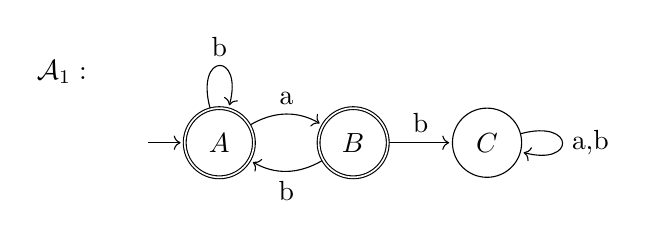
\begin{tikzpicture}[shorten >=1pt, node distance=1.7cm, on grid, auto, initial text=]
                \node at (-2,.9) {$\mathcal{A}_1:$};
                \node[state, initial, accepting] (A)   {$A$};
                \node[state, accepting] (B) [right=of A] {$B$};
                \node[state] (C) [right=of B] {$C$};
                \path[->]
                (A) edge[bend left, above] node {a} (B)
                (A) edge[loop above] node {b} ()
                (B) edge[bend left, below] node {b} (A)
                (B) edge[] node {b} (C)
                (C) edge[loop right] node {a,b} ();
        \end{tikzpicture}\\
        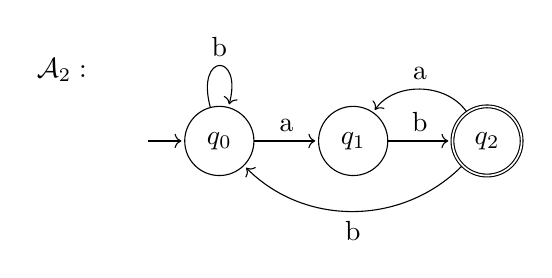
\begin{tikzpicture}[shorten >=1pt, node distance=1.7cm, on grid, auto, initial text=]
                \node at (-2,.9) {$\mathcal{A}_2:$};
                \node[state, initial] (q_0)   {$q_0$};
                \node[state] (q_1) [right=of q_0] {$q_1$};
                \node[state, accepting] (q_2) [right=of q_1] {$q_2$};
                \path[->]
                (q_0) edge[loop above] node {b} ()
                (q_0) edge[] node {a} (q_1)
                (q_1) edge[] node {b} (q_2)
                (q_2) edge[bend left=-55, above] node{a} (q_1)
                (q_2) edge[bend left=45] node{b} (q_0);
        \end{tikzpicture}\\
        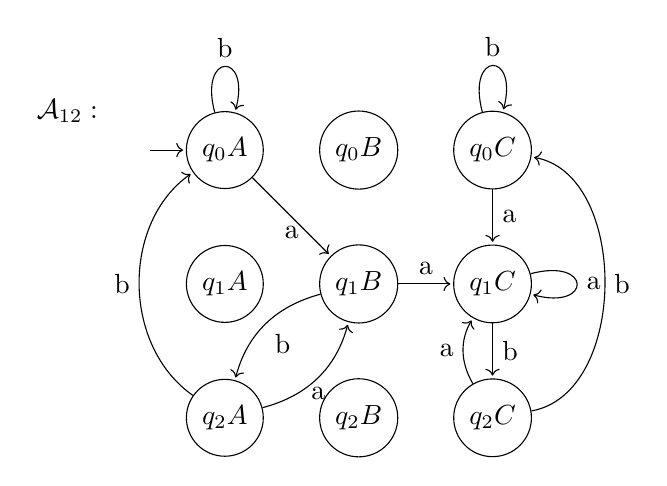
\begin{tikzpicture}[shorten >=1pt, node distance=1.7cm, on grid, auto, initial text=]
                \node at (-2,.5) {$\mathcal{A}_{12}:$};
                \node[state, initial] (q_0A)   {$q_0A$};
                \node[state] (q_0B) [right=of q_0A] {$q_0B$};
                \node[state] (q_0C) [right=of q_0B] {$q_0C$};
                \node[state] (q_1A) [below=of q_0A] {$q_1A$};
                \node[state] (q_1B) [below=of q_0B] {$q_1B$};
                \node[state] (q_1C) [below=of q_0C] {$q_1C$};
                \node[state] (q_2A) [below=of q_1A] {$q_2A$};
                \node[state] (q_2B) [below=of q_1B] {$q_2B$};
                \node[state] (q_2C) [below=of q_1C] {$q_2C$};
                \path[->]
                (q_0A) edge[loop above] node {b} ()
                (q_0A) edge[below] node {a} (q_1B)
                (q_2A) edge[bend left=55] node {b} (q_0A)
                (q_2A) edge[bend right, below] node {a} (q_1B)
                (q_1B) edge[bend right] node {b} (q_2A)
                (q_1B) edge[above] node {a} (q_1C)
                (q_0C) edge[loop above] node {b} ()
                (q_0C) edge[] node {a} (q_1C)
                (q_1C) edge[loop right] node {a} ()
                (q_1C) edge[] node {b} (q_2C)
                (q_2C) edge[bend left] node {a} (q_1C)
                (q_2C) edge[bend right=80,right] node {b} (q_0C);
        \end{tikzpicture}
        \vspace{15pt}
        \\Affinché l'automa $\mathcal{A}_{12}$ riconosca $L_1 \cap L_2$, dobbiamo impostare come stati finali gli stati che sono finali in $\mathcal{A}_1$ e $\mathcal{A}_2$ quindi $q_2A$ e $q_2B$.  Affinché riconosca $L_1 \cup L_2$, dobbiamo impostare come stati finali gli stati che sono finali in $\mathcal{A}_1$ o $\mathcal{A}_2$ quindi $q_0A, q_1A, q_2A, q_0B, q_1B, q_2B, q_2A, q_2B, q_2C$ e affinché riconosca $L_1 \setminus L_2$ dobbiamo impostare come stati finali gli stati che sono finali in $\mathcal{A}_1$ ma non $\mathcal{A}_2$, quindi $q_0A,q_1A,q_0B,q_1B$.

        \subsubsection{Pumping lemma per FSA}
        Sia $L$ un linguaggio riconosciuto da un FSA, allora $\exists p \in \mathbb{N}^+$ tale che ogni stringa $w \in L$ con $|w| \geq p$ può essere scritta come $w = xyz$ con:
        \begin{enumerate}[left=3pt, itemsep=-1pt]
                \item $|xy| \leq p$
                \item $y \neq \upvarepsilon$
                \item $\forall i \geq 0, xy^iz \in L$
        \end{enumerate}
        \textbf{Esempio} Dimostriamo che il linguaggio $L = \{0^n1^n | n \geq 0\}$ non è riconosciuto da un FSA usando il pumping lemma.
        \begin{enumerate}[left=3pt, itemsep=0pt]
                \item Supponiamo per assurdo che $L$ sia riconosciuto da un FSA e scegliamo $w = 0^p1^p$
                \item Scomponiamo $w$ in $xyz$ con:
                      \begin{enumerate}[left=0pt, topsep=0pt, label=\tiny\textbullet]
                              \item $|xy| \leq p$
                              \item $|y| \geq 1$
                      \end{enumerate}
                      Scegliamo $x=0^\alpha, y=0^\beta, z=0^{p-\alpha-\beta}1^p$ con $\alpha \geq 0,\ \beta \geq 1,\ \alpha + \beta \leq p$
                \item Troviamo $i \geq 0$ tale che $xy^iz \notin L$
                      \begin{enumerate}[left=-3pt, topsep=0pt, label=]
                              \item $xy^iz = 0^\alpha0^{i\beta}0^{p-\alpha-\beta}1^p = 0^{p+i\beta-\beta}1^p$. Da cui abbiamo $xy^iz \in L \iff p+i\beta-\beta = p \iff i = 1$. Scegliendo quindi $i \neq 1$, ad esempio $i = 0$, abbiamo che $xy^iz \notin L$ che contraddice la nostra supposizione iniziale. \qed
                      \end{enumerate}
        \end{enumerate}
        \subsection{Automi a pila (AP/PDA)}
        Formalmente definiti come una settupla $(Q,I,\Gamma,\delta,q_0,Z_0,F)$ dove $Q$ è un insieme finito di stati, $I$ è l'alfabeto di input, $\Gamma$  l'alfabeto di pila, $\delta : Q \times (I \cup \{\upvarepsilon\}) \times \Gamma \rightarrow Q \times \Gamma^*$ è la funzione di transizione, che mappa lo stato corrente, un simbolo $I \in I$ e il simbolo $\gamma \in \Gamma$ in cima alla pila a un nuovo stato e una nuova stringa $\gamma' \in \Gamma^*$ che sostituisce la cima della pila, $q_0 \in Q$ è lo stato di partenza, $Z_0$ è il simbolo che denota il fondo della pila e $F \subseteq Q$ è l'insieme degli stati finali.
        \subsubsection{PDA riconoscitore}
        Un linguaggio $L$ è riconosciuto da un PDA se e solo se $\forall s \in L$, dopo aver scandito la stringa $s$, si trova in uno stato $q_f \in F$. \\ [3pt]
        \textbf{Esempio} Automa a pila che riconosce il linguaggio $L=\{a^nb^n \mid n>0\}$ \\ [3pt]
        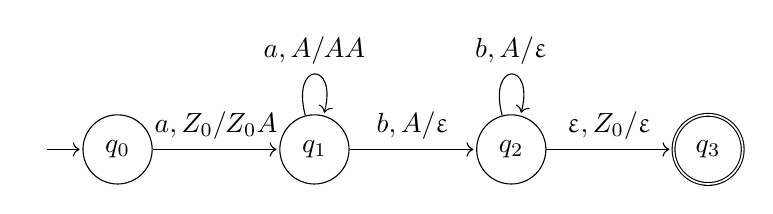
\begin{tikzpicture}[shorten >=1pt, node distance=2.5cm, on grid, auto, initial text=]
                \node[state, initial] (q_0)   {$q_0$};
                \node[state] (q_1) [right=of q_0] {$q_1$};
                \node[state] (q_2) [right=of q_1] {$q_2$};
                \node[state, accepting] (q_3) [right=of q_2] {$q_3$};
                \path[->]
                (q_0) edge node { $a, Z_0/Z_0A$ } (q_1)
                (q_1) edge [loop above] node { $a, A/AA$ } ()
                edge node { $b, A/\upvarepsilon$ } (q_2)
                (q_2) edge [loop above] node { $b, A/\upvarepsilon$ } ()
                edge node { $\upvarepsilon, Z_0/\upvarepsilon$ } (q_3);
        \end{tikzpicture} \\ [3pt]
        $\upvarepsilon, Z_0/\upvarepsilon$ è una $\upvarepsilon$-mossa, cioè una mossa che non consuma simboli in ingresso.
        \subsubsection{PDA traduttore}
        Un PDA traduttore è dotato di un nastro di uscita su cui può scrivere ad ogni transizione.
        \subsection{Macchine di Turing (MT/TM)}
        Le macchine di Turing a $k$ nastri di memoria sono macchine dotate di un nastro di input e $k$ nastri di memoria. Sono formalmente definite come una settupla $(Q,I,\Gamma,$\blank$,\delta,q_0,F)$ dove $Q, I, q_0, F$ sono gli stessi di un PDA/FSA, $\Gamma$ è l'alfabeto di nastro, \blank $\ \in \Gamma$ denota una cella di nastro vuota e $\delta:Q \times (I \cup \{$\blank$\}) \times \Gamma^k \rightarrow Q \times \Gamma^k \times \{L,S,R\}^{k+1}$ è la funzione di transizione dove $L_i,S_i,R_i$ denotano il movimento dell testina sull'$i$-esimo nastro ($k+1$ perché oltre ai $k$ nastri di memoria ci si può muovere anche sul nastro di input). Le macchine di Turing a nastro singolo sono un modello di calcolo equivalente alle macchine di Turing a $k$ nastri dove input e memoria si trovano su un unico nastro.\\[3pt]
        \textbf{Def.} Una macchina di Turing universale (MTU) è una macchina di Turing in grado di simulare qualsiasi altra macchina di Turing. \\ [3pt]
        \subsubsection{MT riconoscitore}
        Una MT riconosce il linguaggio $L$ se per ogni stringa $w \in L$ si ferma in uno stato di accettazione in un numero finito di transizioni. \\ [3pt]
        \textbf{Esempio} Macchina di Turing a $k=1$ nastro di memoria che riconosce il linguaggio $L=\{a^nb^nc^n \mid n>0\}$ \\ [3pt]
        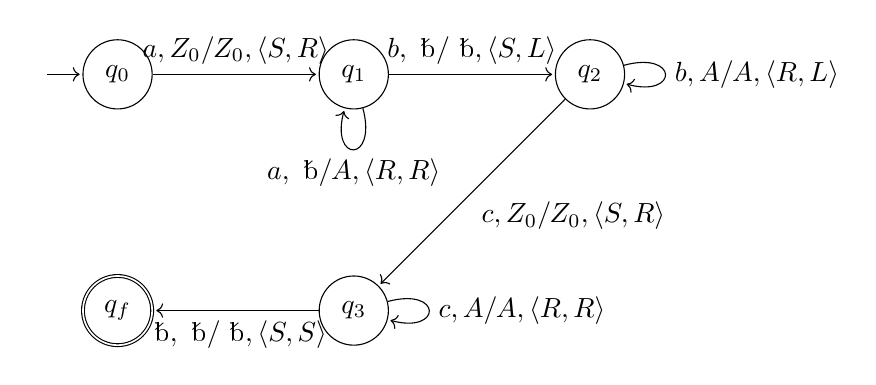
\begin{tikzpicture}[shorten >=1pt, node distance=3cm, on grid, auto, initial text=]
                \node[state, initial] (q0)   {$q_0$};
                \node[state] (q1) [right=of q0] {$q_1$};
                \node[state] (q2) [right=of q1] {$q_2$};
                \node[state] (q3) [below=of q1] {$q_3$};
                \node[state, accepting] (qf) [left=of q3] {$q_f$};
                \path[->]
                (q0) edge node { $a, Z_0/Z_0, \langle S, R \rangle$ } (q1)
                (q1) edge [loop below] node { $a, \text{ \blank}/A, \langle R, R \rangle$ } ()
                edge node { $b, \text{ \blank}/\text{ \blank}, \langle S, L \rangle$ } (q2)
                (q2) edge [loop right] node { $b, A/A, \langle R, L \rangle$ } ()
                (q3) edge [loop right] node { $c, A/A, \langle R, R \rangle$ } ()
                (q2) edge node { $c, Z_0/Z_0, \langle S, R \rangle$ } (q3)
                (q3) edge node { $\text{ \blank}, \text{ \blank}/\text{ \blank}, \langle S, S \rangle$ } (qf);
        \end{tikzpicture} \\ [3pt]
        L'esempio utilizza la convenzione della MT infinita a destra con il simbolo $Z_0$ che denota la prima cella del nastro di memoria.
        \subsubsection{MT traduttore}
        Una MT trad. è dotata di un addizionale nastro di output su cui può solo scrivere e in cui la testina può muoversi solo a destra (\verb|R|) o stare ferma (\verb|S|).
        \subsection{Non determinismo}
        Informalmente, un modello di calcolo si dice non deterministico se esiste almeno una configurazione da cui è possibile prendere più di una strada. Gli FSA e le MT non deterministici hanno le stesse capacità espressive della loro versione deterministica. Gli automi a pila non deterministici (NPDA), invece, sono più espressivi di quelli deterministici. Per esempio, possono riconoscere $L = \{a^nb^n\} \cup \{a^nb^{2n}\}$. Dato un FSA non deterministico con insieme di stati $Q$, è possibile ricavare la sua versione non deterministica con un numero di stati che è al più $2^{|Q|}$ usando la \textit{costruzione per sottoinsiemi} (\textit{powerset construction}).\\ [3pt]
        \textbf{Esempio} \\ [3pt]
        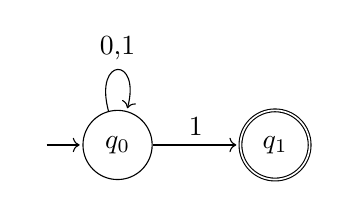
\begin{tikzpicture}[baseline=(current bounding box.center), shorten >=1pt, node distance=2cm, on grid, auto, initial text=]
                \node[state, initial] (q_0) {$q_0$};
                \node[state, accepting] (q_1) [right=of q_0] {$q_1$};
                \path[->]
                (q_0) edge[loop above] node {0,1} ()
                (q_0) edge[] node {1} (q_1);
        \end{tikzpicture}
        \hspace{9pt}$\iff$\hspace{8pt}
        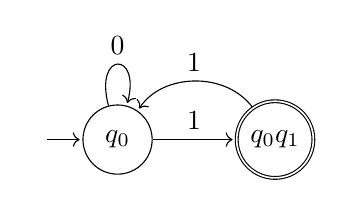
\begin{tikzpicture}[baseline=(current bounding box.center), shorten >=1pt, node distance=2cm, on grid, auto, initial text=]
                \node[state, initial] (q_0) {$q_0$};
                \node[state, accepting] (q_0q_1) [right=of q_0] {$q_0q_1$};
                \path[->]
                (q_0) edge[loop above] node {0} ()
                (q_0q_1) edge[bend left=-55, above] node {1} (q_0)
                (q_0) edge[] node {1} (q_0q_1);
        \end{tikzpicture}
        \subsection{Macchine RAM}
        Le macchine RAM sono un modello di calcolo equivalente alle macchine di Turing. Hanno un nastro di lettura \texttt{In} e uno di scrittura \texttt{Out} e sono dotate di memoria infinita con accesso a indirizzamento diretto. Supportano le seguenti istruzioni:\\[3pt]
        \begin{tabular}{r l  l l}
                \verb|READ X|   & M[X] $\leftarrow$ \texttt{In}         & \verb|WRITE* X| & \texttt{Out} $\leftarrow$ M[M[X]] \\
                \verb|READ* X|  & M[M[X]]   $\leftarrow$ \texttt{In}    & \verb|JUMP l|   & \texttt{PC} $\leftarrow l$        \\
                \verb|LOAD X|   & M[0] $\leftarrow$ M[X]                & \verb|JZ l|     & se M[0]=0                         \\
                \verb|LOAD= X|  & M[0]   $\leftarrow$ X                 &                 & \texttt{PC} $\leftarrow l$        \\
                \verb|LOAD* X|  & M[0]   $\leftarrow$ M[M[X]]           & \verb|JGT l|    & se M[0]$>$0                       \\
                \verb|STORE X|  & M[X] $\leftarrow$ M[0]                &                 & \texttt{PC} $\leftarrow l$        \\
                \verb|STORE* X| & M[X]   $\leftarrow$ M[M[0]]           & \verb|JGZ l|    & se M[0]$\geq$0                    \\
                \verb|ADD X|    & M[0]  $\leftarrow$ M[0] + M[X]        &                 & \texttt{PC} $\leftarrow l$        \\
                \verb|SUB X|    & M[0]  $\leftarrow$ M[0] - M[X]        & \verb|JLT l|    & se M[0]$<$0                       \\
                \verb|MUL X|    & M[0]  $\leftarrow$ M[0] $\times$ M[X] &                 & \texttt{PC} $\leftarrow l$        \\
                \verb|DIV X|    & M[0]  $\leftarrow$ M[0] / M[X]        & \verb|JLZ l|    & se M[0]$\leq$0                    \\
                \verb|WRITE X|  & \texttt{Out} $\leftarrow$ M[X]        &                 & \texttt{PC} $\leftarrow l$        \\
                \verb|WRITE= X| & \texttt{Out} $\leftarrow$ X           & \verb|HALT|     & termina exec.                     \\
        \end{tabular}
        \subsection{Logica monadica del I ordine (MFO)}
        La logica monadica del I ordine è un modello di calcolo in grado di riconoscere linguaggi star-free, ossia linguaggi regolari esprimibili senza l'utilizzo della star di Kleene. La sintassi di una formula $\varphi$ della logica monadica del I ordine è  $\varphi := a(x) \ | \ x < y \ | \ \lnot \varphi \ | \ \varphi \land \varphi \ | \ \forall x (\varphi)$ \\
        Dove $x,y \in \mathbb{N}$, $a(x)$ è un predicato unario che è vero se e solo se alla posizione $x$ c'è il simbolo $a$ e $<$ è un predicato binario che corrisponde alla relazione di minore. Partendo da questi assiomi si può definire il connettivo $\lor$, il quantificatore esistenziale $\exists$, le relazioni aritmetiche $=, \leq, >, \geq$ e somme e sottrazioni tra variabili e costanti ($y=x \pm k$). Si possono inoltre definire abbreviazioni ausiliarie, come:\\
        \begin{tabular}{r l}
                \verb|last(x)| & $\lnot \exists y (y>x)$ \\
                \verb|y=S(x)|  & $y=x+1$                 \\
        \end{tabular}
        \subsection{Logica monadica del II ordine (MSO)}
        La logica monadica del II ordine è un modello di calcolo con le stesse capacità espressive degli automi a stati finiti. Differisce da MFO per il fatto che consente la quantificazione su insiemi di posizioni. \\
        \textbf{Esempio} La seguente formula della logica monadica del II ordine riconosce il linguaggio $L = \{a^{2n}\ |\ n \in \mathbb{N}^+\}$.\\ [5pt]
        $\exists P (\forall x(a(x) \land \lnot P(0) \land \forall y(y=x+1 \implies (\lnot P(x) \iff P(y))) \land (last(x) \implies P(x))))$ \\ [5pt]
        Dove $X(x)$ significa $x \in X$.
        \section{Grammatiche}
        Una grammatica è una quadrupla $G=(T, N, P, S)$ dove $T$ è l'alfabeto terminale, $N$ è l'alfabeto nonterminale, $S \in N$ è il simbolo iniziale e $P \subseteq N^+ \times (N \cup T)^*$ è l'insieme delle produzioni sintattiche. Data una grammatica $G$ si definisce derivazione immediata
        la relazione binaria $\underset{G}{\implies}$ definita come: $x \underset{G}{\implies}y \iff \exists u,v,p,q \in (N \cup T)^*:(x=upv) \land (p \rightarrow q \in P) \land (y=uqv)$ \\ \textbf{Esempio} Prendiamo in considerazione la grammatica $G = \langle \{a,b\}, \{S,R\}, \{S \rightarrow aR,R \rightarrow bS, S \rightarrow \upvarepsilon\}, S\rangle$, abbiamo che $abaR \underset{G}{\implies} ababS$. Il linguaggio $L(G)$ generato dalla grammatica $G$ è l'insieme di tutte e sole le stringhe $s$ di soli caratteri di $T$ tali che

        $S\underset{G}{\overset{*}{\implies}}s$ dove $\underset{G}{\overset{*}{\implies}}$ è la chiusura riflessiva e transitiva di $\underset{G}{\implies}$.
        A seconda delle limitazioni imposte sulle regole di produzione $\alpha \rightarrow \beta$ si hanno 4 tipi di grammatiche \\ [5pt]
        \begin{tabular}{@{}r m{2.5cm} m{2.6cm} l@{}}
                \textbf{Tipo} & \textbf{Nome}                     & \textbf{Regole prod.}                                                                                            & \textbf{Equiv.} \\ \hline
                \verb|0|      & Non ristretta                     & nessuna                                                                                                          & TM              \\ \hline
                \verb|1|      & Monotone oppure Context sensitive & $|\alpha| \leq |\beta|$ oppure $\alpha=\gamma A \delta,\ \beta=\gamma \chi \delta$ con $\chi \neq \upvarepsilon$ & (LBA)           \\ \hline
                \verb|2|      & Context free                      & $|a| = 1$                                                                                                        & NPDA            \\ \hline
                \verb|3|      & Regolare                          & $A \rightarrow \alpha,\ A \rightarrow \alpha A$ o $A \rightarrow \alpha,\ A \rightarrow A\alpha$                 & FSA             \\\hline
        \end{tabular}\\ [5pt]
        Si può dimostrare che le grammatiche monotone e dipendenti dal contesto hanno la stessa capacità espressiva.
        \subsection{Conversione Automa $\leftrightarrow$ Grammatica}
        Dato un automa $\mathcal{A}$ che riconosce un certo linguaggio $L(\mathcal{A})$, è possibile ricavare la grammatica $\mathcal{G}$ tale che $L(\mathcal{G})=L(\mathcal{A})$ (o viceversa). \\ [3pt]
        \textbf{Esempio FSA} Linguaggio $L=(ab)^*a(ab)^*$\\
        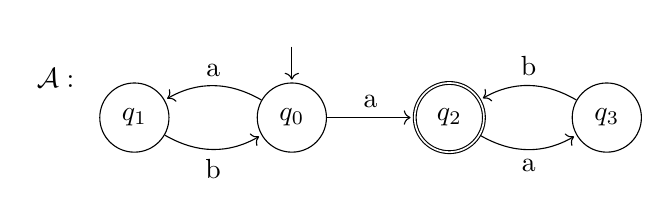
\begin{tikzpicture}[shorten >=1pt, node distance=2cm, on grid, auto, initial text=]
                \node at (-3,.5) {$\mathcal{A}:$};
                \node[state, initial above] (q_0) {$q_0$};
                \node[state, accepting] (q_2) [right=of q_0] {$q_2$};
                \node[state] (q_1) [left=of q_0] {$q_1$};
                \node[state] (q_3) [right=of q_2] {$q_3$};
                \path[->]
                (q_0) edge[] node {a} (q_2)
                (q_2) edge[bend right, below] node {a} (q_3)
                (q_3) edge[bend right, above] node {b} (q_2)
                (q_0) edge[bend right, above] node {a} (q_1)
                (q_1) edge[bend right, below] node {b} (q_0);
        \end{tikzpicture}\\
        $\mathcal{G} = (T=\{a,b\},N=\{q_0,q_1,q_2,q_3\},P,S=q_0)$ \\
        \begin{tabular}{@{}ll}
                $P:$ & $q_0 \rightarrow aq_1|aq_2|a$ \\
                     & $q_1 \rightarrow bq_0$        \\
                     & $q_2 \rightarrow aq_3$        \\
                     & $q_3 \rightarrow bq_2|b$      \\
        \end{tabular}
        \subsection{Proprietà di chiusura dei linguaggi}
        \begin{minipage}{\textwidth}
                \bgroup
                \def\arraystretch{1}% 
                \begin{tabular}{r c c c c c c c}
                                                & \textbf{REG} & \textbf{DCFL} & \textbf{CFL} & \textbf{CSL} & \textbf{RIC} & \textbf{RE} \\ \hline
                        \texttt{Unione}         & \checkmark   & $\times$      & \checkmark   & \checkmark   & \checkmark   & \checkmark  \\\hline
                        \texttt{Intersezione}   & \checkmark   & $\times$      & $\times$     & \checkmark   & \checkmark   & \checkmark  \\\hline
                        \texttt{Differenza}     & \checkmark   & $\times$      & $\times$     & \checkmark   & \checkmark   & $\times$    \\\hline
                        \texttt{Complemento}    & \checkmark   & \checkmark    & $\times$     & \checkmark   & \checkmark   & $\times$    \\\hline
                        \texttt{Concatenazione} & \checkmark   & $\times$      & \checkmark   & \checkmark   & \checkmark   & \checkmark  \\\hline
                        \texttt{Star di Kleene} & \checkmark   & $\times$      & \checkmark   & \checkmark   & \checkmark   & \checkmark  \\\hline
                \end{tabular}
                \egroup
                \vspace{5pt}
        \end{minipage}
        \begin{tabular}{@{}r p{7.6cm}@{}}
                \verb|REG|  & Linguaggi regolari (riconosciuti da una grammatica regolare / esprimibili mediante un'espressione regolare) \\
                \verb|DCFL| & Linguaggi context free deterministici (riconosciuti da una grammatica context free deterministica)          \\
                \verb|CFL|  & Linguaggi context free (riconosciuti da una grammatica context free)                                        \\
                \verb|CSL|  & Linguaggi context sensitive (riconosciuti da una grammatica context sensitive)                              \\
                \verb|RIC|  & Linguaggi ricorsivi (esiste una MT che per ogni stringa appartenente al linguaggio, accetta o rifiuta)      \\
                \verb|RE|   & Linguaggi ricorsivamente enumerabili (riconosciuti da una grammatica non ristretta)                         \\
        \end{tabular} \\ [5pt]
        \verb|FIN| (linguaggi finiti) $\subset$ \verb|REG| $\subset$ \verb|DCFL| $\subset$ \verb|CFL| $\subset$ \verb|CSL| $\subset$ \verb|RIC| $\subset$ \verb|RE|\\ [3pt]
        \section{Teoria della computazione}
        \begin{tabular}{@{}r p{6.5cm}@{}}
                \verb|Tesi di Church| & tutti i problemi computabili sono descrivibili da una macchina di Turing. \textit{(MT, programma, algoritmo, procedura sono usati come sinonimi)}                                                     \\
                \verb|problema|       & richiesta di calcolo algoritmico di $f:A\rightarrow B$ con $|A|,|B| \leq |\mathbb{N}|$. (In generale $f$ è parziale, cioè $\exists n(f(n)=\bot)$)                                                     \\
                \verb|f. computabile| & se esiste un algoritmo che calcola $f$, $f$ è calcolabile e il problema è computabile. $f_i$ denota l'$i$-esima funzione computabile. \textit{(calcolabile, computabile e risolvibile sono sinonimi)} \\
                \verb|ins. dec.|      & un insieme $S$ è decidibile (o ricorsivo) se esiste una funzione $\mathbbm{1}_S$ che restituisce 1 se $n \in S$ e 0 se $n \notin S$.                                                                  \\
                \verb|ins. semidec.|  & un insieme $S$ è semidecidibile (o ricorsivamente enumerabile o r.e.) se esiste una funzione $\mathbbm{1}'_S(n)$ che restituisce 1 se $n \in S$.                                                      \\
        \end{tabular} \\[3pt]
        Se un problema è chiuso, cioè che la sua soluzione non dipende da un valore in ingresso, allora è decidibile. \\[3pt]
        \textbf{Teorema} Sia $S$ un insieme, allora:\\ $S \text{ ric. } \iff S \text{ r.e.} \land S^C \text{ r.e.}$ \\ [3pt]
        \textbf{Corollario} Se $\lnot S$ ric., allora: \\
        $(S \text{ r.e.} \land \lnot S^C \text{ r.e.}) \lor (\lnot S \text{ r.e.} \land S^C \text{ r.e.}) \lor (\lnot S \text{ r.e.} \land \lnot S^C \text{ r.e.})$
        \subsection{Dimostrazione di semidecidibiltà (Dovetailing)}
        Per stabilire se $\exists z \mid f_x(z) \neq \bot$ si può usare la tecnica del \textit{dovetailing} che consiste nell'eseguire una sola mossa alla volta per ogni input fin quando non ci si arresta. Se $\exists z \mid f_x(z) \neq \bot$ sicuramente prima o poi viene incontrato e ci si arresta. Non si possono eseguire in sequenza $f_x(0)$ e poi $f_x(1)$ e così via perché se $f_x(0) = \bot$ non si arriverà mai ad eseguire $f_x(1)$.\\ [3pt]
        \columnbreak
        \subsection{Teorema di Rice}
        Sia $F = \{f_i\ |\ i \in \mathbb{N}\}$ l'insieme di tutte le funzioni computabili, sia $P \subseteq F = \{f_i\ |\ f_i\text{ soddisfa una certa proprietà}\}$ un sottoinsieme di $F$ di funzioni computabili che soddisfano una certa proprietà e sia \\$S=\{x\ |\ f_x \in P\}$ l'insieme degli indici delle funzioni che appartengono a $P$. Allora $S$ ric. $\iff P = \varnothing \lor P = F$. Più informalmente, il teorema di Rice afferma che per qualsiasi proprietà non banale (cioè vera per almeno una funzione e falsa per almeno una funzione) delle funzioni computabili, non esiste un algoritmo che possa decidere se una data funzione computabile soddisfi o meno quella proprietà.
                \subsection{Riduzione}
                La riduzione può essere usata per dimostrare che un dato problema è decidibile o indecidibile.\\
                \textbf{Caso decidibile} Sia $P_1$ un noto problema decidibile e sia $P_2$ un problema che si sospetta essere decidibile. Si può dimostrare che $P_2$ è decidibile riducendolo a $P_1$.\\[3pt]
                \textsc{RisolviP$_2$}($x$)\\
                \hspace*{1.5em}$y \leftarrow \textsc{Riduci}(x)$\\
                \hspace*{1.5em}$sol \leftarrow \textsc{RisolviP$_1$}(y)$\\
                \hspace*{1.5em}\textbf{return} $sol$\\[3pt]
                \textbf{Caso indecidibile} Sia $P_1$ un noto problema indecidibile e sia $P_2$ un problema che si sospetta essere indecidibile. Si può dimostrare che $P_2$ è indecidibile riducendolo da $P_1$.\\[3pt]
                \textsc{RisolviP$_1$}($x$)\\
                \hspace*{1.5em}$y \leftarrow \textsc{Riduci}(x)$\\
                \hspace*{1.5em}$sol \leftarrow \textsc{RisolviP$_2$}(y)$\\
                \hspace*{1.5em}\textbf{return} $sol$\\[3pt]
                In altre parole, se riuscissimo a risolvere $P_2$, riusciremmo a risolvere anche $P_1$ ma questo è impossibile in quanto $P_1$ è un noto problema indecidibile.
                \subsection{Noti problemi indecidibili}
                \subsubsection{Problema dell'arresto (Halting problem)}
                Data una macchina di Turing $\mathcal{M}$ e un input $w$, determinare se $\mathcal{M}$ si arresta su $w$.\\ [3pt]
        $H = \{ \langle \mathcal{M}, w \rangle \mid \mathcal{M} \text{ si arresta sull'input } w \}$
                \subsubsection{Problema dell'equivalenza delle MT}
                Date due macchine di Turing $\mathcal{M}_1$ e $\mathcal{M}_2$, determinare se calcolano la stessa funzione.\\ [3pt]
        $EQ = \{ \langle \mathcal{M}_1, \mathcal{M}_2 \rangle \mid \mathcal{M}_1 \text{ e } \mathcal{M}_2 \text{ calcolano la stessa funzione} \}$
                \subsubsection{Problema della totalità delle MT}
                Data una macchina di Turing $\mathcal{M}$, determinare se $\mathcal{M}$ si arresta su tutti gli input.\\ [3pt]
        $TOT = \{ \langle \mathcal{M} \rangle \mid \mathcal{M} \text{ si arresta su tutti gli input} \}$
                \subsubsection{Problema del linguaggio vuoto}
                Data una macchina di Turing $\mathcal{M}$, determinare se il linguaggio riconosciuto da $\mathcal{M}$ è vuoto.\\ [3pt]
        $E = \{ \langle \mathcal{M} \rangle \mid L(\mathcal{M}) = \varnothing \}$\\ [3pt]
                \section{Analisi di complessità degli algoritmi}
                \subsection{Formule note}
        $\sum_{i=1}^{n} i = \frac{n(n+1)}{2}$\hfill$\sum_{i=1}^{n} i^2 = \frac{n(n+1)(2n+1)}{6}$\hfill$\sum_{i=1}^{n} i^3 = \frac{n^2(n+1)^2}{4}$\\[3pt]$\sum_{i=1}^{n} x^i = \frac{x^{n+1}-1}{x-1}$\hfill$\sum_{i=1}^{\infty} x^i = \frac{1}{1-x}\ (\text{se } |x|<1) $\hfill$\sum_{i=1}^{n} \log(i)=\log(n!)$\\[5pt]
                \textbf{Stirling approx.} $n! \sim \sqrt{2 \pi n} (\frac{n}{e})^n$ per $n \rightarrow \infty$. Da questo si può dimostrare che $\log(n!) \overset{n \rightarrow \infty}{\sim} n\log n$.
                \subsection{Definizioni di $O$-grande, $\Omega$-grande, $\Theta$-grande}
                \subsubsection{$O$-grande}
        $O(g(n))$ è l'insieme delle funzioni che sono asintoticamente dominate da $g(n)$ a meno di una costante.\\[5pt]
        $O(g(n)) = \{f(n)\ |\ \exists c>0, n_0>0 \text{ tali che } \forall n \geq n_0, f(n) \leq c\cdot g(n)$\}
                \subsubsection{$\Omega$-grande}
        $\Omega(g(n))$ è l'insieme delle funzioni che dominano asintoticamente $g(n)$ a meno di una costante.\\[5pt]
        $\Omega(g(n)) = \{f(n)\ |\ \exists c>0, n_0>0 \text{ tali che } \forall n \geq n_0, f(n) \geq c\cdot g(n)$\}
                \subsubsection{$\Theta$-grande}
        $\Theta(g(n))$ è l'insieme delle funzioni che hanno approssimativamente lo stesso comportamento astintotico di $g(n)$.\\[5pt]
        $\Theta(g(n)) = \{ f(n)\ |\ \exists c_1 > 0, c_2 > 0, n_0 > 0 \text{ tali che } \forall n \geq n_0, \ c_1 \cdot g(n) \leq f(n) \leq c_2 \cdot g(n) \}$
                \\[5pt]
                \textbf{N.B.} Spesso si utilizza la notazione $f(n) = O(g(n))$ invece di $f(n) \in O(g(n))$ per indicare che la funzione $f(n)$ appartiene all'insieme di funzioni $O(g(n))$ anche se non è una notazione formalmente corretta.
                \subsection{Criterio di costo costante e logaritmico}
                Nella valutazione della complessità algoritmica con criterio di costo costante, ogni istruzione ha costo $\Theta(1)$. Con il criterio di costo logaritmico, invece, leggere (\texttt{READ}), copiare (\texttt{LOAD}), spostare (\texttt{STORE}), scrivere (\texttt{WRITE}), eseguire somme (\texttt{ADD}) e sottrazioni (\texttt{SUB}) ha costo $\Theta(\log(n))$, eseguire moltiplicazioni (\texttt{MUL}) e divisioni (\texttt{DIV}) ha costo $\Theta(\log^2(n))$ e il resto (\texttt{JUMP/HALT}) ha costo $\Theta(1)$. \\ [5pt]
                \textbf{Esempio} Calcolo di $2^{2^{n}}$ con macchina RAM con criterio di costo logaritmico.\\[5pt]
                \begin{tabular}{r l |l}
                        \texttt{1}  & \texttt{READ 2}       & $\log(n)$                                        \\
                        \texttt{2}  & \texttt{LOAD= 2}      & $\log(2) = k$                                    \\
                        \texttt{3}  & \texttt{STORE 1}      & $\log(2) = k$                                    \\
                        \texttt{4}  & \texttt{loop: LOAD 1} & $\log(2^{2^n-1}) = 2^{n-1}$                      \\
                        \texttt{5}  & \texttt{MUL 1}        & $(\log(2^{2^{n-1}}))^2 = (2^{n-1})^2 = 2^{2n-2}$ \\
                        \texttt{6}  & \texttt{STORE 1}      & $\log(2^{2n}) = 2n$                              \\
                        \texttt{7}  & \texttt{LOAD 2}       & $\log(n)$                                        \\
                        \texttt{8}  & \texttt{SUB= 1}       & $\log(n)$                                        \\
                        \texttt{9}  & \texttt{STORE 2}      & $\log(n-1)$                                      \\
                        \texttt{10} & \texttt{JGT loop}     & 1                                                \\
                        \texttt{11} & \texttt{WRITE 1}      & $\log(2^{2^n}) = 2^n$                            \\
                        \texttt{12} & \texttt{HALT}         & 1                                                \\
                \end{tabular}\\[5pt]
        $T(n)=\log(n)+n(2^{n-1}+2^{2n-2}+2^n+3\log(n))+2^n = \Theta(n2^{2n-2})$
                \subsection{Ricorrenze}
                \subsubsection{Master theorem}
                Data l'equazione di ricorrenza $T(n)=aT(\frac{n}{b})+f(n)$ con $a \geq 1, b > 1$.
                \[
                        T(n) =
                        \begin{cases}
                                \Theta(n^{\log_b{a}})        & \text{se } f(n) = O(n^c) \text{ con } c < \log_ba                                            \\
                                \Theta(n^{\log_b{a}} \log n) & \text{se } f(n) = \Theta(n^{\log_ba})                                                        \\
                                \Theta(f(n))                 & \text{se } f(n) = \Omega(n^c) \text{ con } c > \log_ba \text{ e } af(\frac{n}{b}) \leq kf(n)
                        \end{cases}
                \]
                Per qualche $k < 1$.\\ [3pt]
                \myparagraph{Generalizzazione del caso 2}
                Se $f(n)=\Theta(n^{\log_ba}\log^kn)$ per qualche $k \in \mathbb{R}$, allora: \\ [5pt]
                \[
                        T(n) =
                        \begin{cases}
                                \Theta(n^{\log_ba}\log^{k+1}n) & \text{se } k > -1 \\
                                \Theta(n^{\log_ba} \log\log n) & \text{se } k = -1 \\
                                \Theta(n^{\log_ba})            & \text{se } k < -1
                        \end{cases}
                \]\\[6pt]
                Notiamo che se $k=0$ ci troviamo nel caso semplice visto sopra.
                \subsubsection{Sostituzione}
                Consiste nell'intuire una soluzione, sostituirla nell'equazione di ricorrenze $T(n)$ e verificare che esistano $c$ e $n_0$ che rispettino la definizione di $O$-grande.\\ [3pt]
                \textbf{Esempio} Consideriamo $T(n) = 3T(\log(n))+2^n$. Intuiamo che $T(n)=O(2^n)$. Verifichiamo che esistano $c>0, n_0 > 0$ tale che $\forall n \geq n_0,\ T(n) \leq c2^n$ da cui segue che $T(\log(n)) \leq c2^{logn} = cn$\\$T(n)=3T(\log(n))+2^n \leq 3cn+2^n \leq \frac{c}{2}2^n+2^n = (\frac{c}{2}+1)2^n \overset{?}{\leq} c2^n$. Sì, basta prendere $c \geq 2. \qed$\\[3pt]
                L'intuizione per la $O$-grande si può ottenere espandendo le chiamate ricorsive e individuando il termine dominante o trovando due funzioni tra cui $T(n)$ è compresa.  In generale, per dimostrare che $T(n) \in \Theta(f(n))$ bisogna dimostrare che $T(n) \in O(f(n))$ e che $T(n) \in \Omega(f(n))$ in modo analogo a quanto visto nell'esempio.
                \section{Strutture dati}
                \subsection{Vettori}
                I vettori sono strutture dati che consentono l'accesso diretto ad ogni elemento data la sua posizione.\\ [5pt]
                \begin{tabular}{r|p{4cm}|l}
                        Operazione       & Non ord.                                                 & Ord.              \\
                        \hline
                        \verb|Search|    & $O(n)$                                                   & $\Theta(\log(n))$ \\
                        \verb|Minimum|   & $O(n)$                                                   & $\Theta(1)$       \\
                        \verb|Maximum|   & $O(n)$                                                   & $\Theta(1)$       \\
                        \verb|Successor| & $O(n)$                                                   & $\Theta(\log(n))$ \\
                        \verb|Insert|    & $O(n)$                                                   & $O(n)$            \\
                        \verb|Delete|    & $O(n)$ (oppure $O(1)$ usando dei simboli di cella vuota) & $O(n)$            \\
                \end{tabular} \\ [5pt]
                L'inserimento in un vettore pieno può essere rifiutato $O(1)$ o può causare una riallocazione $O(n)$.
                \subsection{Liste}
                Le liste semplici sono strutture dati che memorizzano elementi sparsi in memoria dove ogni elemento contiene un riferimento al successivo. \\ [3pt]
                \begin{tabular}{r|l|l}
                        Operazione       & Non ord. & Ord.                      \\
                        \hline
                        \verb|Search|    & $O(n)$   & $O(n)$                    \\
                        \verb|Minimum|   & $O(n)$   & $\Theta(1)$ o $\Theta(n)$ \\
                        \verb|Maximum|   & $O(n)$   & $\Theta(n)$ o $\Theta(1)$ \\
                        \verb|Successor| & $O(n)$   & $O(n)$                    \\
                        \verb|Insert|    & $O(1)$   & $O(n)$                    \\
                        \verb|Delete|    & $O(n)$   & $O(n)$                    \\
                \end{tabular} \\ [3pt]
                A seconda di come è ordinata la lista, uno tra \verb|Minimum| e \verb|Maximum| è $\Theta(1)$ e l'altro è $\Theta(n)$.
                \subsubsection{Pile (Stack)}
                Le pile sono strutture dati con le seguenti operazioni:\\[3pt]
                \begin{tabular}{rl}
                        \verb|Push(S,e)| & aggiunge l'elemento \verb|e| in cima alla pila \verb|S| \\
                        \verb|Pop(S)|    & restituisce e cancella l'elemento in cima alla pila     \\
                        \verb|Empty(S)|  & restituisce \verb|true| se la pila è vuota              \\
                \end{tabular}\\ [3pt]
                \myparagraph{Implementazione con vettori}
                Possono essere implementate con dei vettori memorizzando l'indice della cima della pila (Top of Stack, ToS). \\ [3pt]
                \begin{tabular}{rl}
                        \verb|Push(S,e)| & se c'è spazio incrementa ToS e salva \verb|e| in \verb|A[ToS]|  $O(1)$ \\
                                         & altrimenti rifiuta $O(1)$ o rialloca $O(n)$                            \\
                        \verb|Pop(S)|    & restituisce \verb|A[ToS]| e decrementa \verb|ToS|               $O(1)$ \\
                        \verb|Empty(S)|  & restituisce \verb|true| se \verb|ToS=0|                         $O(1)$ \\
                \end{tabular}
                \myparagraph{Implementazione con liste}
                Possono essere implementate con delle liste dove la testa della lista è la cima della pila. \\ [3pt]
                \begin{tabular}{rl}
                        \verb|Push(S,e)| & inserisce \verb|e| in testa alla lista                             $O(1)$ \\
                        \verb|Pop(S)|    & restituisce e cancella l'elemento in testa alla lista              $O(1)$ \\
                        \verb|Empty(S)|  & restituisce \verb|true| se il successore della testa è \verb|NIL| $O(1)$  \\
                \end{tabular}

                \subsubsection{Code (Queues)}
                Le code sono strutture dati con le seguenti operazioni:\\[3pt]
                \begin{tabular}{rl}
                        \verb|Enqueue(Q,e)| & aggiunge l'elemento \verb|e| alla fine della coda \verb|Q| \\
                        \verb|Dequeue(Q)|   & restituisce e cancella l'elemento all'inizio della coda    \\
                        \verb|Empty(Q)|     & restituisce \verb|true| se la coda è vuota                 \\
                \end{tabular}\\ [3pt]
                \myparagraph{Implementazione con vettori}
                Possono essere implementate con dei vettori tenendo traccia della posizione dove va inserito un nuovo elemento e di quella dell'elemento più vecchio con due indici \verb|tail| e \verb|head| e del numero di elementi contenuti $n$. Sia $A$ il vettore e $l := A.length$  \\ [3pt]
                \begin{tabular}{rl}
                        \verb|Enqueue(Q,e)| & se $n < l$ salva \verb|e| in \verb|A[tail]| e incrementa $n$ e \verb|tail|  $O(1)$ \\
                                            & altrimenti rifiuta $O(1)$ o rialloca $\Theta(n)$                                   \\
                        \verb|Dequeue(Q)|   & restituisce \verb|A[head]|, decrementa $n$ e incrementa \verb|head|        $O(1)$  \\
                        \verb|Empty(Q)|     & restituisce \verb|true| se $n=0$                                           $O(1)$  \\
                \end{tabular}
                \myparagraph{Implementazione con liste}
                Possono essere implementate con delle liste tenendo traccia sia della testa (\verb|head|) che della coda (\verb|tail|) della lista. \\ [3pt]
                \begin{tabular}{rl}
                        \verb|Enqueue(Q,e)| & inserisce l'elemento \verb|e| in coda alla lista       $O(1)$ \\
                        \verb|Dequeue(Q)|   & restituisce e cancella l'elemento in testa alla lista  $O(1)$ \\
                        \verb|Empty(Q)|     & restituisce \verb|true| se \verb|head=tail|            $O(1)$ \\
                \end{tabular}

                \subsubsection{Code doppie (Double-ended queues o Deques)}
                Le code doppie sono strutture dati in cui è possibile inserire sia in testa che in coda. Sono dotate delle seguenti operazioni: \\ [3pt]
                \begin{tabular}{rl}
                        \verb|PushFront(Q,e)| & inserisce l'elemento \verb|e| in testa      \\
                        \verb|PushBack(Q,e)|  & inserisce l'elemento \verb|e| in coda       \\
                        \verb|PopFront(Q)|    & restituisce e cancella l'elemento in testa  \\
                        \verb|PopBack(Q)|     & restituisce e cancella l'elemento in coda   \\
                        \verb|Empty(Q)|       & restituisce \verb|true| se la deque è vuota \\
                \end{tabular}
                \myparagraph{Implementazione con vettori}
                \verb|PushBack|, \verb|PopFront| e \verb|Empty| sono analoghi a \verb|Enqueue| e \verb|Dequeue| della coda realizzata con vettore. \\ [3pt]
                \begin{tabular}{rl}
                        \verb|PushFront(Q,e)| & se $n<l$ decr. \verb|head|, ins. \verb|e| in \verb|A[head]| e incr. $n$ $O(1)$ \\
                                              & altrimenti segnala l'errore $O(1)$                                             \\
                        \verb|PopBack(Q)|     & se $n>0$, restituisce \verb|A[tail]| e decr. $n$ e \verb|tail|  $O(1)$         \\
                \end{tabular}
                \myparagraph{Implementazione con liste \textit{doppiamente concatenate}}
                \verb|PushBack| e \verb|PopFront| sono analoghi a \verb|Enqueue| e \verb|Dequeue| della coda realizzata con lista. Una lista vuota è rappresentata con \verb|head| e \verb|tail| che puntano l'uno all'altro.\\ [3pt]
                \begin{tabular}{rl}
                        \verb|PushFront(Q,e)| & ins. \verb|e| in testa aggiornando \verb|head| e il suo succ.  $O(1)$     \\
                        \verb|PopBack(Q)|     & restituisce e cancella \verb|tail.prev|                            $O(1)$ \\
                        \verb|Empty(Q)|       & se $n>0$, restituisce \verb|true| se \verb|head.next=tail|         $O(1)$ \\
                \end{tabular}

                \subsection{Dizionari}
                I dizionari sono strutture dati che contengono elementi accessibili direttamente data la loro chiave. Supportano le operazioni: \verb|Insert|, \verb|Delete|, \verb|Search| e sono implementati come vettori di puntatori dove le chiavi vengono usate come indici del vettore. \\ [3pt]
                \begin{tabular}{rll}
                        \verb|Insert(D,e)|     & \verb|D[e.key]| $\leftarrow$ \verb|e|   & $\Theta(1)$ \\
                        \verb|Delete(D,e)|     & \verb|D[e.key]| $\leftarrow$ \verb|NIL| & $\Theta(1)$ \\
                        \verb|Search(D,e.key)| & \textbf{return} \verb|D[e.key]|         & $\Theta(1)$ \\
                \end{tabular}\\ [3pt]
                La complessità spaziale è $O(|\textbf{D}|)$ con $\textbf{D}$ il dominio delle chiavi.
                \subsubsection{Tabelle di hash}
                Una tabella di hash è un caso speciale di dizionario con una complessità spaziale pari al numero di chiavi $m$ per cui è effettivamente presente un valore. L'indice associato a una certa chiave è dato dal risultato di una funzione $h(\cdot):\textbf{D} \rightarrow \{0,\dots,m-1\}$ detta funzione di hash. \\[3pt]
                \textbf{Def.} Il fattore di carico $\alpha$ è definito come $\frac{n}{m}$ dove $n$ è il numero di elementi contenuti nella tabella e $m$ è il numero di righe totali.
                \myparagraph{Collisioni}
                Date due chiavi $k_1,k_2$ con $k_1 \neq k_2$ abbiamo una collisione se $h(k_1)=h(k_2)$. Le collisioni si  risolvono principalmente con due metodi.
                \myparagraph{Indirizzamento chiuso (closed addressing/open hashing/chaining)}
                Ogni riga della tabella (bucket) contiene la testa di una lista. Nel caso di collisione, l'elemento viene inserito in testa alla lista $\Theta(1)$. Nel caso peggiore tutti gli elementi collidono dando origine a una lista lunga $m$ elementi, quindi \verb|Insert/Delete/Search| in $O(m)$. \\ [3pt]
                \textbf{Def.} Ipotesi di Hashing Uniforme Semplice (IHUS) è un'oppurtuna funzione di hash dove ogni chiave ha probabilità $\frac{1}{m}$ di finire in una qualsiasi delle $m$ celle.\\ [3pt]
                In caso di IHUS, la lunghezza media di una listà è $\alpha$ e il tempo medio per cercare una chiave è $\Theta(1+\alpha)$. Se $\alpha$ non è eccessivo, tutte le operazioni sono $O(1)$ in media. Per mantenere l'efficienza delle operazioni, si sceglie un $\alpha$ oltre il quale viene fatta una riallocazione in una tabella più grande (\textbf{rehashing}). (i solito $\alpha_{max} \simeq 0.75$)
                \myparagraph{Indirizzamento aperto (open addressing/closed hashing)}
                \verb|Insert|: Consiste nel selezionare deterministicamente l'indirizzo di un altro bucket in caso di collisione (ispezione). Se non ci sono bucket liberi, l'inserimento fallisce $\Theta(m)$ e viene fatto il rehashing. Si modifica \verb|Search| affinché effettui la stessa ispezione in caso l'elemento non sia presente nel suo bucket. \verb|Delete| si effettua inserendo un opportuno valore (tombstone) che non corrisponde ad alcuna chiave. \\ [3pt]\textbf{Complessità} Sotto IHUS, cercare un valore non presente costa $\Theta(\frac{1}{1-\alpha})$, mentre cercare un valore presente costa $\Theta(\frac{1}{\alpha} \log (\frac{1}{1-\alpha}))$.\\ [3pt]
                \textbf{Ispezione lineare (linear probing)}: Si sceglie $h(k,i)=a+c\cdot i \mod m$ come candidato per l'$i$-esimo inserimento. \\
                Se ci sono molte collisioni in un bucket, aumenta la probabilità di collisione nelle vicinanze (\textbf{clustering primario}). \\ [3pt]
                \textbf{Ispezione quadratica (quadratic probing)}: Si sceglie $h(k,i)=a+c_1i+c_2i^2 \mod m$ come candidato per l'$i$-esimo inserimento. Rimuove il clustering primario ma non garantisce che tutte le celle vengano toccate dalla sequenza di ispezione. \\ [3pt]
                \textbf{Doppio hashing} (passo di ispezione dipende dalla chiave) $h(k,i)=h_1(k)+h_2(k)i$. Per garantire che tutte le celle vengano toccate dalla sequenza di ispezione $h_2(k)$ deve essere coprimo con $m$. In particolare:
                \begin{enumerate}[left=1em, itemsep=0.5pt, label=\raisebox{0.5ex}{\tiny$\bullet$}]
                        \item $m = 2^x \leftrightarrow h_2$ genera solo num. dispari
                        \item $m$ primo $\leftrightarrow h_2$ genera numero $<m$
                        \item $h_2$ non  deve mai restituire $0$ altrimenti la sequenza di ispezione degenera
                \end{enumerate}
                \textbf{Esempio}
                Sia $T$ una tabella di hash con $31$ celle e $\alpha = 3/4$. Vogliamo reindirizzare i dati in una tabella $T'$ di modo che $\alpha' \le 1/2$. Qual è il numero minimo $m'$ di celle che è opportuno che $T'$ abbia? Si assuma che $h_{T'}(k,i)=(k+i(2k+1)) \mod m'$.\\ [3pt]
                \textbf{Sol.} Essendo $h_2(k)$ sempre dispari, scegliamo $m'$ come potenza di $2$ che soddisfi la restrizione imposta su $\alpha'$: \\ [3pt]
                $\alpha'=\frac{\text{\# celle occupate}}{\text{\# celle disponibili}}=\frac{3/4*31}{m'} \le \frac{1}{2} \iff m' \ge \frac{3}{2}*31 = 46.5$ \\ [3pt]
                Scegliamo quindi $m' = 64$.
                \myparagraph{Aritmetica modulare}
        $\frac{a}{n}$ stesso resto di $\frac{r}{n} \iff a \equiv r\mod n \iff  n \mid (a-r) \iff a = qn+r$.  \\ [3pt]
                \textbf{Proprietà} \\ [3pt]
        $(a \pm b)\mod n= [(a\mod n) \pm (b\mod n)]\mod n$ \\ [3pt]
        $(a \times b)\mod n = [(a\mod n) \times (b\mod n)]\mod n$ \\
                \subsection{Alberi}
                Un albero è una struttura dati rappresentata da una coppia (\textbf{V},\textbf{E}) con \textbf{V} insieme di nodi e \textbf{E} insieme di archi dove ogni nodo può apparire un'unica volta come destinazione di un arco. \\ [3pt]
                \textbf{Definizioni} \\ [3pt]
                \begin{tabular}{rp{7cm}}
                        \verb|radice|          & l'unico nodo privo di un arco entrante                                                                                                           \\
                        \verb|foglia|          & nodo senza archi uscenti                                                                                                                         \\
                        \verb|padre| di $n$    & nodo da cui l'arco entrante in $n$ ha origine                                                                                                    \\
                        \verb|figlio| di $n$   & nodo in cui uno degli archi uscenti da $n$ termina                                                                                               \\
                        \verb|livello|         & distanza di un nodo dalla radice                                                                                                                 \\
                        \verb|albero completo| & albero in cui tutti i livelli hanno tutti i nodi tranne l'ultimo che può non avere tutti i nodi ma i nodi devono essere più a sinistra possibile \\
                \end{tabular}
                \subsubsection{Alberi binari}
                Un albero binario è un albero in cui ogni nodo ha al più due figli. Dato un nodo \verb|A|: \\ [3pt]
                \begin{tabular}{rlrl}
                        \verb|A.left| & ref. a figlio sinistro & \verb|A.right| & ref. a figlio destro \\
                        \verb|A.p|    & ref. al padre          & \verb|A.root|  & ref. alla radice     \\
                \end{tabular} \\ [3pt]
                \verb|A.p| è \verb|NIL| solo per la radice.
                \myparagraph{Implementazione con vettore}
                \begin{multicols}{2}
                        \begin{center}
                                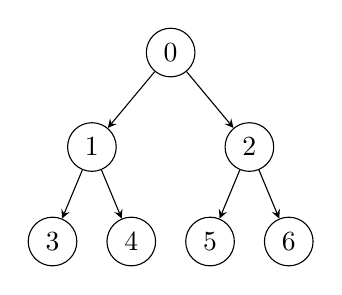
\begin{tikzpicture}[
                                                ->,
                                                >=stealth,
                                                level/.style={sibling distance = 2cm/#1, level distance = 1.2cm},
                                                every node/.style={circle, draw, minimum size=6mm}
                                        ]
                                        \node [circle,draw] (z){0}
                                        child {node [circle,draw] (a) {1}
                                                        child {node [circle,draw] (b) {3}}
                                                        child {node [circle,draw] (c) {4}}
                                                }
                                        child {node [circle,draw] (d) {2}
                                                        child {node [circle,draw] (e) {5}}
                                                        child {node [circle,draw] (f) {6}}
                                                };
                                \end{tikzpicture} \\ [7pt]

                                \renewcommand\arraystretch{1.5}
                                \begin{tabular}{|c|c|c|c|c|c|c|}
                                        \hline
                                        \multicolumn{1}{|c|}{0} & \multicolumn{1}{c|}{1} & \multicolumn{1}{c|}{2} & \multicolumn{1}{c|}{3} & \multicolumn{1}{c|}{4} & \multicolumn{1}{c|}{5} & \multicolumn{1}{c|}{6} \\
                                        \hline
                                \end{tabular}
                        \end{center}
                        \begin{itemize}[left=0pt, label=\raisebox{0.5ex}{\tiny$\bullet$}]
                                \item La radice ha indice 0.
                                \item Dato un nodo con indice $i$, il suo figlio sinistro ha indice $2i+1$ e il suo figlio destro ha indice $2i+2$
                                \item Il padre del nodo con indice $i$ ha indice $\lfloor\frac{i-1}{2}\rfloor$
                        \end{itemize}
                \end{multicols}
                \myparagraph{Visita di un albero}
                Le principali procedure di visita di un albero sono \textsc{InOrder}, \textsc{PreOrder} e \textsc{PostOrder}.
                \begin{multicols}{3}
                        \textsc{InOrder($T$)}\\ [3pt]
                        \verb|1|\hspace*{0.5em}\textbf{if} $T \neq$ \verb|NIL|\\
                        \verb|2|\hspace*{1.2em}\textsc{InOrder($T.left$)}\\
                        \verb|3|\hspace*{1.2em}\textsc{Print($T.key$)}\\
                        \verb|4|\hspace*{1.2em}\textsc{InOrder($T.right$)}\\
                        \verb|5|\hspace*{0.5em}\textbf{return}\\ [5pt]
                        $3,1,4,0,5,2,6$\\
                        \columnbreak
                        \textsc{PreOrder($T$)}\\ [3pt]
                        \verb|1|\hspace*{0.5em}\textbf{if} $T \neq$ \verb|NIL|\\
                        \verb|2|\hspace*{1.2em}\textsc{Print($T.key$)}\\
                        \verb|3|\hspace*{1.2em}\textsc{PreOrder($T.left$)}\\
                        \verb|4|\hspace*{1.2em}\textsc{PreOrder($T.right$)}\\
                        \verb|5|\hspace*{0.5em}\textbf{return}\\  [5pt]
                        $0,1,3,4,2,5,6$\\
                        \columnbreak
                        \textsc{PostOrder($T$)}\\ [3pt]
                        \verb|1|\hspace*{0.5em}\textbf{if} $T \neq$ \verb|NIL|\\
                        \verb|2|\hspace*{1.2em}\textsc{PostOrder($T.left$)}\\
                        \verb|3|\hspace*{1.2em}\textsc{PostOrder($T.right$)}\\
                        \verb|4|\hspace*{1.2em}\textsc{Print($T.key$)}\\
                        \verb|5|\hspace*{0.5em}\textbf{return}\\  [5pt]
                        $3,4,1,5,6,2,0$\\
                \end{multicols}
                Tutte queste procedure hanno complessità temporale $\Theta(n)$ in quanto toccano ogni nodo dell'albero esattamente una volta.
                \subsubsection{Alberi binari di ricerca (BST)}
                Un albero binario di ricerca è un albero binario che, per ogni nodo $x$, soddisfa le sequenti condizioni:
                \begin{itemize}[left=1em, label=\raisebox{0.5ex}{\tiny$\bullet$}]
                        \item Se $y$ è contenuto nel sottoalbero sinistro di $x$, allora $y.key \leq x.key$
                        \item Se $y$ è contenuto nel sottoalbero destro di $x$, allora $y.key \geq x.key$
                \end{itemize}
                \textbf{Esempi} \\ [3pt]
                \noindent
                \begin{multicols}{2}
                        \centering
                        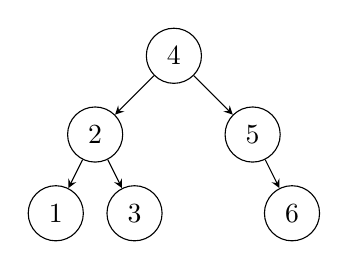
\begin{tikzpicture}[
                                        ->,
                                        >=stealth,
                                        level/.style={sibling distance=2cm/#1, level distance=1cm},
                                        every node/.style={circle, draw, minimum size=7mm},
                                ]
                                \node (z) {4}
                                child {node (a) {2}
                                                child {node (b) {1}}
                                                child {node (c) {3}}
                                        }
                                child {node (d) {5}
                                                child[missing] {}
                                                child {node (f) {6}}
                                        };
                        \end{tikzpicture}
                        \columnbreak
                        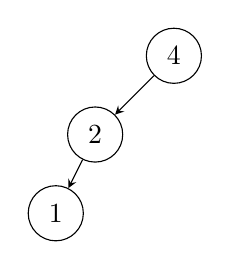
\begin{tikzpicture}[
                                        ->,
                                        >=stealth,
                                        level/.style={sibling distance=2cm/#1, level distance=1cm},
                                        every node/.style={circle, draw, minimum size=7mm},
                                ]
                                \node (z) {4}
                                child {node (a) {2}
                                                child {node (b) {1}}
                                                child [missing] {}
                                        }
                                child [missing] {};
                        \end{tikzpicture}
                \end{multicols}
                \myparagraph{Operazioni su BST}
                \begin{multicols}{2}
                        \textsc{Search($T,x$)} $:\ O(h)$\\ [3pt]
                        \verb|1|\hspace*{0.5em} \textbf{if} $T=$ \verb|NIL| or $T.key=x.key$\\
                        \verb|2|\hspace*{1.5em} \textbf{return} $T$\\
                        \verb|3|\hspace*{0.5em} \textbf{if} $T.key<x.key$\\
                        \verb|4|\hspace*{1.5em} \textbf{return} \textsc{Search}($T.right,x$)\\
                        \verb|5|\hspace*{0.5em} \textbf{else return} \textsc{Search}($T.left,x$)\\
                        \columnbreak
                        \textsc{Min($T$)} $:\ O(h)$\\ [3pt]
                        \verb|1|\hspace*{0.5em} $cur \leftarrow T$\\
                        \verb|2|\hspace*{0.5em} \textbf{while} $cur.left \neq$ \verb|NIL|\\
                        \verb|3|\hspace*{1.5em} $cur \leftarrow cur.left$\\
                        \verb|4|\hspace*{0.5em} \textbf{return} $cur$\\
                \end{multicols}
                \begin{multicols}{2}
                        \textsc{Max($T$)} $:\ O(h)$\\ [3pt]
                        \verb|1|\hspace*{0.5em} $cur \leftarrow T$\\
                        \verb|2|\hspace*{0.5em} \textbf{while} $cur.right \neq$ \verb|NIL|\\
                        \verb|3|\hspace*{1.5em} $cur \leftarrow cur.right$\\
                        \verb|4|\hspace*{0.5em} \textbf{return} $cur$\\
                        \columnbreak
                        \textsc{Successor($x$)} $:\ O(h)$\\ [3pt]
                        \verb|1|\hspace*{0.5em} \textbf{if} $x.right \neq$ \verb|NIL|\\
                        \verb|2|\hspace*{1.5em} \textbf{return} \textsc{Min}($x.right$)\\
                        \verb|3|\hspace*{0.5em} $y \leftarrow x.p$\\
                        \verb|4|\hspace*{0.5em} \textbf{while} $y \neq$ \verb|NIL| and $y.right=x$\\
                        \verb|5|\hspace*{1.5em} $x \leftarrow y$\\
                        \verb|6|\hspace*{1.5em} $y \leftarrow y.p$\\
                        \verb|7|\hspace*{0.5em} \textbf{return} $y$\\
                \end{multicols}
                \begin{multicols}{2}
                        \textsc{Insert($T,x$)} $:\ O(h)$\\ [3pt]
                        \verb| 1|\hspace*{0.5em} $pre \leftarrow$ \verb|NIL|\\
                        \verb| 2|\hspace*{0.5em} $cur \leftarrow T.root$\\
                        \verb| 3|\hspace*{0.5em} \textbf{while} $cur \neq$ \verb|NIL|\\
                        \verb| 4|\hspace*{1.5em} $pre \leftarrow cur$\\
                        \verb| 5|\hspace*{1.5em} \textbf{if} $x.key < cur.key$\\
                        \verb| 6|\hspace*{2.5em} $cur \leftarrow cur.left$\\
                        \verb| 7|\hspace*{1.5em} $cur \leftarrow cur.right$\\
                        \verb| 8|\hspace*{0.5em} $x.p \leftarrow pre$\\
                        \verb| 9|\hspace*{0.5em} \textbf{if} $pre =$ \verb|NIL|\\
                        \verb|10|\hspace*{1.5em} $T.root \leftarrow x$\\
                        \verb|11|\hspace*{0.5em} \textbf{elseif} $x.key < pre.key$\\
                        \verb|12|\hspace*{1.5em} $pre.left \leftarrow x$\\
                        \verb|13|\hspace*{0.5em} \textbf{else} $pre.right \leftarrow x$\\
                        \columnbreak
                        \textsc{Delete(T,x)} $:\ O(h)$ \\ [3pt]
                        \verb| 1|\hspace*{0.5em} \textbf{if} $x.left=$ \verb|NIL| or $x.right=$ \verb|NIL|\\
                        \verb| 2|\hspace*{1.5em} $del \leftarrow x$\\
                        \verb| 3|\hspace*{0.5em} \textbf{else} $del \leftarrow$ \textsc{Successor}($x$)\\
                        \verb| 4|\hspace*{0.5em} \textbf{if} $del.left \neq$ \verb|NIL|\\
                        \verb| 5|\hspace*{1.5em} $subtree \leftarrow del.left$\\
                        \verb| 6|\hspace*{0.5em} \textbf{else} $subtree \leftarrow del.right$\\
                        \verb| 7|\hspace*{0.5em} \textbf{if} $subtree \neq$ \verb|NIL|\\
                        \verb| 8|\hspace*{1.5em} $subtree.p \leftarrow del.p$\\
                        \verb| 9|\hspace*{0.5em} \textbf{if} $del.p =$ \verb|NIL|\\
                        \verb|10|\hspace*{1.5em} $T.root \leftarrow subtree$\\
                        \verb|11|\hspace*{0.5em} \textbf{elseif} $del = del.p.left$\\
                        \verb|12|\hspace*{1.5em} $del.p.left \leftarrow subtree$\\
                        \verb|13|\hspace*{0.5em} \textbf{else} $del.p.right \leftarrow subtree$\\
                        \verb|14|\hspace*{0.5em} \textbf{if} $del \neq x$\\
                        \verb|15|\hspace*{1.5em} \textbf{else} $x.key \leftarrow del.key$\\
                        \verb|16|\hspace*{0.5em} \textsc{Free}(del)\\
                \end{multicols}
                La complessità di tutte le operazioni è $O(h)$ con $h$ altezza dell'albero. Nel caso ottimo (albero bilanciato) è $O(\log(n))$, nel caso pessimo (albero degenere in una lista) è $O(n)$.
                \subsubsection{Alberi rosso-neri (Red-black trees / RB trees)}
                Gli alberi rosso-neri sono BST i cui nodi hanno un colore $\in \{\text{rosso, nero}\}$ e che soddisfano le seguenti proprietà:
                \begin{enumerate}[left=1em, itemsep=1pt]
                        \item Ogni nodo è rosso o nero
                        \item La radice è nera
                        \item Le foglie sono nere
                        \item I figli di un nodo rosso sono entrambi neri
                        \item Per ogni nodo dell’albero, tutti i cammini dai suoi discendenti alle foglie contenute nei suoi sottoalberi hanno lo stesso numero di nodi neri
                \end{enumerate}
                Le operazioni che non modificano la struttura dell'albero sono le stesse dei BST (\textsc{Search, Min, Max, Successor}). Le procedure di inserimento (\textsc{Insert}) e cancellazione (\textsc{Delete}) sono modificate per mantenere l'albero bilanciato assicurando una complessità temporale di $O(\log(n))$ per tutte le operazioni.
                \subsubsection{Heap binari}
                Gli heap binari sono alberi binari quasi-completi dove la chiave del nodo padre è sempre maggiore o minore di quella dei figli. Nel primo caso si parla di max-heap nel secondo di min-heap.\\ [3pt]
                \textbf{Esempio (max-heap)} \\ [3pt]
                \begin{center}
                        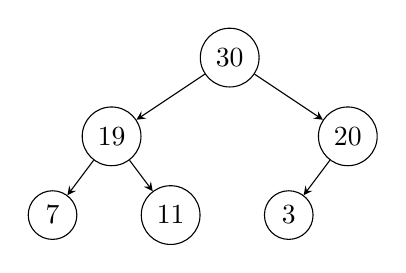
\begin{tikzpicture}[
                                        ->,
                                        >=stealth,
                                        level/.style={sibling distance = 3cm/#1, level distance = 1cm},
                                        every node/.style={circle, draw, minimum size=6mm}
                                ]
                                \node [circle,draw] (z){30}
                                child {node [circle,draw] (a) {19}
                                                child {node [circle,draw] (b) {7}}
                                                child {node [circle,draw] (c) {11}}
                                        }
                                child {node [circle,draw] (d) {20}
                                                child {node [circle,draw] (e) {3}}
                                                child [missing] {}
                                        };
                        \end{tikzpicture} \\ [7pt]
                \end{center}
                \myparagraph{Operazioni su max-heap}
                \textsc{MaxHeapify}($A,n$) riceve un array e una posizione in esso: assume che i due sottoalberi con radice in \textsc{Left}($n$) $= 2n$ e \textsc{Right}($n$) $= 2n + 1$ siano dei max-heap e modifica $A$ in modo che l’albero radicato in $n$ sia un max-heap. \\ [5pt]
                \textsc{MaxHeapify($A,n$)} $:\ O(\log(n))$                                     \\ [3pt]
                \texttt{ 1}\hspace*{0.5em} $l \leftarrow$ \textsc{Left($n$)}                      \\
                \texttt{ 2}\hspace*{0.5em} $r \leftarrow$ \textsc{Right($n$)}                     \\
                \texttt{ 3}\hspace*{0.5em} \textbf{if} $l \leq A.heapsize$ and $A[l] > A[n]$      \\
                \texttt{ 4}\hspace*{1.5em} $posmax \leftarrow l$                                  \\
                \texttt{ 5}\hspace*{0.5em} \textbf{else} $posmax \leftarrow n$                    \\
                \texttt{ 6}\hspace*{0.5em} \textbf{if} $r \leq A.heapsize$ and $A[r] > A[posmax]$ \\
                \texttt{ 7}\hspace*{1.5em} $posmax \leftarrow r$                                  \\
                \texttt{ 8}\hspace*{0.5em} \textbf{if} $posmax \neq n$                            \\
                \texttt{ 9}\hspace*{1.5em} \textsc{Swap}($A[n],A[posmax]$)                        \\
                \texttt{10}\hspace*{1.5em} \textsc{MaxHeapify}($A,posmax$)                       \\ [5pt]
                \begin{multicols}{2}
                        \textsc{BuildMaxHeap($A$)} $:\ O(n)$                                     \\ [3pt]
                        \texttt{1}\hspace*{0.5em} $A.heapsize \leftarrow A.length$                      \\
                        \texttt{2}\hspace*{0.5em} \textbf{for }$i \leftarrow \lfloor\frac{A.length}{2}\rfloor$ \textbf{downto} 1                     \\
                        \texttt{3}\hspace*{1.5em} \textsc{MaxHeapify}($A,i$)      \\
                        \columnbreak
                        \textsc{Max($A$)} $:\ O(1)$ \\ [3pt]
                        \texttt{1}\hspace*{0.5em} \textbf{return} $A[1]$                     \\
                \end{multicols}
                \setlength{\columnsep}{-0.6cm}
                \begin{multicols}{2}
                        \textsc{ExtractMax($A$)} $:\ O(\log(n))$                                     \\ [3pt]
                        \texttt{1}\hspace*{0.5em} \textbf{if} $A.heapsize < 1$                    \\
                        \texttt{2}\hspace*{1.5em} \textbf{return} $\bot$                    \\
                        \texttt{3}\hspace*{0.5em} $max \leftarrow A[i]$       \\
                        \texttt{4}\hspace*{0.5em} $A[1] \leftarrow A[A.heapsize]$      \\
                        \texttt{5}\hspace*{0.5em} $A.heapsize \leftarrow A.heapsize-1$      \\
                        \texttt{6}\hspace*{0.5em} \textsc{MaxHeapify}($A,1$)      \\
                        \texttt{7}\hspace*{0.5em} \textbf{return} $max$      \\
                        \columnbreak
                        \textsc{Insert($A,key$)} $:\ O(\log(n))$                                     \\ [3pt]
                        \texttt{1}\hspace*{0.5em} $A.heapsize \leftarrow A.heapsize+1$                    \\
                        \texttt{2}\hspace*{0.5em} $A[A.heapsize] \leftarrow key$                    \\
                        \texttt{3}\hspace*{0.5em} $i \leftarrow A.heapsize$       \\
                        \texttt{4}\hspace*{0.5em} \textbf{while} $i > 1$ and $A[\textsc{Parent($i$)}] < A[i]$      \\
                        \texttt{5}\hspace*{1.5em} \textsc{Swap}($A[\textsc{Parent($i$)}],A[i]$)     \\
                        \texttt{6}\hspace*{1.5em} $i \leftarrow \textsc{Parent($i$)}$       \\
                \end{multicols}
                \subsection{Grafi}
                Un grafo è una coppia $\mathcal{G} = (\textbf{V},\textbf{E})$ con \textbf{V} un insieme di nodi (detti anche vertici) ed \textbf{E} un insieme di archi (detti anche lati). \\ [3pt]
                \textbf{Def.} \\
                \begin{itemize}[left=0.7em, label=\raisebox{0.5ex}{\tiny$\bullet$}]
                        \item Un grafo con $|\textbf{V}|$ nodi ha al più $|\textbf{V}|^2$ archi
                        \item Due nodi collegati da un arco si dicono \textit{adiacenti}
                        \item Un grafo è detto \textit{orientato} (directed) se gli archi (arcs) che collegano i nodi sono orientati
                        \item Un grafo è detto \textit{connesso} se esiste un percorso per ogni coppia di nodi
                        \item Un grafo è detto \textit{completo} (o \textit{completamente connesso}) se esiste un arco per ogni coppia di nodi.
                        \item Un percorso è un \textit{ciclo} se il nodo di inizio e fine coincidono. Un grafo privo di cicli si dice \textit{aciclico}
                        \item Un \textit{cammino} tra due nodi $v_1,v_2$ è un insieme di archi di cui il primo ha origine in $v_1$, l’ultimo termina in $v_2$ e ogni nodo compare almeno una volta sia come destinazione di un arco che come sorgente
                \end{itemize}
                \textbf{Esempio} Cammino $v_3 \to v_4: (v_3,v_2), (v_2,v_4)$\\ [3pt]
                \begin{multicols}{2}
                        \begin{center}
                                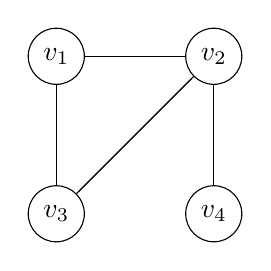
\begin{tikzpicture}[->,>=stealth',shorten >=1pt,auto,node distance=2cm,
                                                main node/.style={circle,draw,minimum size=6mm,font=\normalsize}]
                                        \node[main node] (v1) {$v_1$};
                                        \node[main node] (v2) [right of=v1] {$v_2$};
                                        \node[main node] (v3) [below of=v1] {$v_3$};
                                        \node[main node] (v4) [below of=v2] {$v_4$};

                                        \path[-]
                                        (v1) edge node {} (v2)
                                        (v1) edge node {} (v3)
                                        (v2) edge node {} (v3)
                                        (v2) edge node {} (v4)
                                        (v2) edge node {} (v1)
                                        (v3) edge node {} (v1)
                                        (v3) edge node {} (v2)
                                        (v4) edge node {} (v2);
                                \end{tikzpicture}
                                \columnbreak
                                \begin{itemize}[left=0pt, label=]
                                        \item $\textbf{V} = \{v_1,v_2,v_3,v_4\}$
                                        \item $\textbf{E} = \{(v_1,v_2),(v_1,v_3),(v_2,v_3),$\\
                                              $(v_2,v_4),(v_2,v_1),(v_3,v_1),(v_3,v_2),(v_4,v_2)\}$
                                \end{itemize}
                        \end{center}
                \end{multicols}
                \subsubsection{Rappresentazione in memoria}
                I grafi vengono rappresentati in memoria con \textit{liste di adiacenza} o \textit{matrice di adiacenza}. \\
                \myparagraph{Liste di adiacenza}
                Vettore di liste lungo $|\textbf{V}|$, indicizzato dai nomi dei nodi dove ogni lista contiene i nodi adiacenti all'indice della sua testa.\\ [5pt]
                \begin{center}
                        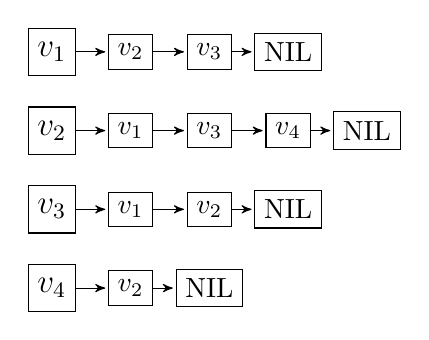
\begin{tikzpicture}[
                                        node distance=1cm,
                                        main/.style={rectangle, draw, minimum size=6mm},
                                        node/.style={rectangle, draw, minimum size=4mm},
                                        null/.style={rectangle, draw, minimum size=4mm},
                                        ->,>=stealth',shorten >=1pt,auto
                                ]

                                % Define the main nodes
                                \node[main] (n0) {\large$v_1$};
                                \node[main, below of=n0] (n1) {\large$v_2$};
                                \node[main, below of=n1] (n2) {\large$v_3$};
                                \node[main, below of=n2] (n3) {\large$v_4$};

                                % Define the adjacent nodes for node 0
                                \node[node, right of=n0] (n0a) {$v_2$};
                                \node[node, right of=n0a] (n0b) {$v_3$};
                                \node[null, right of=n0b] (n0null) {NIL};

                                % Define the adjacent nodes for node 1
                                \node[node, right of=n1] (n1a) {$v_1$};
                                \node[node, right of=n1a] (n1b) {$v_3$};
                                \node[null, right of=n1b] (n1c) {$v_4$};
                                \node[null, right of=n1c] (n1null) {NIL};

                                % Define the adjacent nodes for node 2
                                \node[node, right of=n2] (n2a) {$v_1$};
                                \node[node, right of=n2a] (n2b) {$v_2$};
                                \node[null, right of=n2b] (n2null) {NIL};

                                % Define the adjacent nodes for node 3
                                \node[node, right of=n3] (n3a) {$v_2$};
                                \node[null, right of=n3a] (n3null) {NIL};

                                % Draw the arrows
                                \draw[->] (n0) -- (n0a);
                                \draw[->] (n0a) -- (n0b);
                                \draw[->] (n0b) -- (n0null);

                                \draw[->] (n1) -- (n1a);
                                \draw[->] (n1a) -- (n1b);
                                \draw[->] (n1b) -- (n1c);
                                \draw[->] (n1c) -- (n1null);

                                \draw[->] (n2) -- (n2a);
                                \draw[->] (n2a) -- (n2b);
                                \draw[->] (n2b) -- (n2null);

                                \draw[->] (n3) -- (n3a);
                                \draw[->] (n3a) -- (n3null);
                        \end{tikzpicture}
                \end{center}
                \myparagraph{Matrice di adiacenza}
                Matrice $|\textbf{V}| \times |\textbf{V}|$ di valori booleani con righe e colonne indicizzate dai nomi dei nodi dove la cella alla riga $i$ e colonna $j$ contiene $1$ se l'arco $(v_i,v_j) \in \textbf{E}$ e $0$ altrimenti.\\
                {\large
                \[
                        \renewcommand{\arraystretch}{1.3}%
                        \begin{blockarray}{ccccc}
                                & v_1 & v_2 & v_3 & v_4  \\ [2.5pt]
                                \begin{block}{c(cccc)}
                                        v_1 & 0 & 1 & 1 & 0  \\
                                        v_2 & 1 & 0 & 1 & 1  \\
                                        v_3 & 1 & 1 & 0 & 0  \\
                                        v_4 & 0 & 1 & 0 & 0  \\
                                \end{block}
                        \end{blockarray}
                \]}\\ [5pt]
                \subsubsection{Confronto}
                \renewcommand{\arraystretch}{1.3}%
                \begin{tabular}{r|l|l}
                                                                   & Liste                               & Matrice                  \\
                        \hline
                        Complessità spaziale                       & $\Theta(|\textbf{V}|+|\textbf{E}|)$ & $\Theta(|\textbf{V}|^2)$ \\
                        \hline
                        Determinare se $(v_1, v_2) \in \textbf{E}$ & $O(|\textbf{V}|)$                   & $O(1)$                   \\
                        \hline
                        Num. di archi $o_e$ uscenti da un nodo     & $\Theta(o_e)$                       & $O(|\textbf{V}|)$
                \end{tabular}\\ [5pt]
                Se il grafo è denso, cioè $|\textbf{E}| \approx |\textbf{V}|^2$, è conveniente usare la matrice di adiacenza. Se il grafo è sparso, cioè $|\textbf{E}| \ll |\textbf{V}|^2$, è conveniente usare le liste di adiacenza.
                \columnbreak
                \myparagraph{Operazioni su grafi}
                \textbf{Visita in ampiezza (BFS o Breadth-first search)}\\ [3pt]
                La strategia di visita in ampiezza visita tutti i nodi di un grafo $\mathcal{G}$ a partire da un nodo sorgente $s$. I nodi vengono visitati in ordine di distanza, dove i nodi più vicini al nodo sorgente vengono visitati per primi. \\ [5pt]
                \textsc{VisitaAmpiezza($G,s$)} $:\ O(|\textbf{V}|+|\textbf{E}|)$\\ [3pt]
                \verb| 1|\hspace*{0.5em} $\textbf{for each } n \in \textbf{V} \setminus \{s\}$\\
                \verb| 2|\hspace*{1.5em} $n.color \leftarrow white$\\
                \verb| 3|\hspace*{1.5em} $n.dist \leftarrow \infty$\\
                \verb| 4|\hspace*{0.5em} $s.color \leftarrow grey$\\
                \verb| 5|\hspace*{0.5em} $s.dist \leftarrow 0$\\
                \verb| 6|\hspace*{0.5em} $Q \leftarrow \varnothing$\\
                \verb| 7|\hspace*{0.5em} \textsc{Enqueue($Q,s$)}\\
                \verb| 8|\hspace*{0.5em} \textbf{while} $\lnot \textsc{IsEmpty($Q$)}$\\
                \verb| 9|\hspace*{1.5em} $cur \leftarrow \textsc{Dequeue($Q$)}$\\
                \verb|10|\hspace*{1.5em} $\textbf{for each } v \in cur.adiacenti$\\
                \verb|11|\hspace*{2.5em} $\textbf{if } v.color = white$\\
                \verb|12|\hspace*{3.5em} $v.color \leftarrow grey$\\
                \verb|13|\hspace*{3.5em} $v.dist \leftarrow cur.dist+1$\\
                \verb|14|\hspace*{3.5em} \textsc{Enqueue($Q,v$)}\\
                \verb|15|\hspace*{1.5em} $cur.color \leftarrow black$\\ [5pt]
                \textbf{Visita in profondità (DFS o Depth-first search)}\\ [3pt]
                La strategia di visita in ampiezza visita tutti i nodi di un grafo $\mathcal{G}$ a partire da un nodo sorgente $s$. I nodi vengono visitati in profondità, cioè che si visita un nodo fino a quando non si raggiungono i nodi più lontani (in profondità) rispetto al nodo sorgente. Il codice è uguale a quello per il BFS usando una pila invece che una coda.\\ [5pt]
                \textsc{VisitaProfondità($G,s$)} $:\ O(|\textbf{V}|+|\textbf{E}|)$\\ [3pt]
                \verb| 1|\hspace*{0.5em} $\textbf{for each } n \in \textbf{V} \setminus \{s\}$\\
                \verb| 2|\hspace*{1.5em} $n.color \leftarrow white$\\
                \verb| 3|\hspace*{1.5em} $n.dist \leftarrow \infty$\\
                \verb| 4|\hspace*{0.5em} $s.color \leftarrow grey$\\
                \verb| 5|\hspace*{0.5em} $s.dist \leftarrow 0$\\
                \verb| 6|\hspace*{0.5em} $S \leftarrow \varnothing$\\
                \verb| 7|\hspace*{0.5em} \textsc{Push($S,s$)}\\
                \verb| 8|\hspace*{0.5em} \textbf{while} $\lnot \textsc{IsEmpty($S$)}$\\
                \verb| 9|\hspace*{1.5em} $cur \leftarrow \textsc{Pop($S$)}$\\
                \verb|10|\hspace*{1.5em} $\textbf{for each } v \in cur.adiacenti$\\
                \verb|11|\hspace*{2.5em} $\textbf{if } v.color = white$\\
                \verb|12|\hspace*{3.5em} $v.color \leftarrow grey$\\
                \verb|13|\hspace*{3.5em} $v.dist \leftarrow cur.dist+1$\\
                \verb|14|\hspace*{3.5em} \textsc{Push($S,v$)}\\
                \verb|15|\hspace*{1.5em} $cur.color \leftarrow black$\\ [5pt]
                \textbf{Componenti connesse}\\ [3pt]
                Una \textit{componente connessa} di un grafo è un insieme $\textbf{S}$ di nodi tali per cui esiste
                un cammino tra ogni coppia di essi e nessuno di essi è connesso a nodi  $\notin \textbf{S}$.\\ [5pt]
                \textbf{Esempio} Componenti connesse $S_1 = \{v_1,v_2,v_3,v_4\}, S_2 = \{v_5,v_6,v_7\}$ \\ [3pt]
                \begin{center}
                        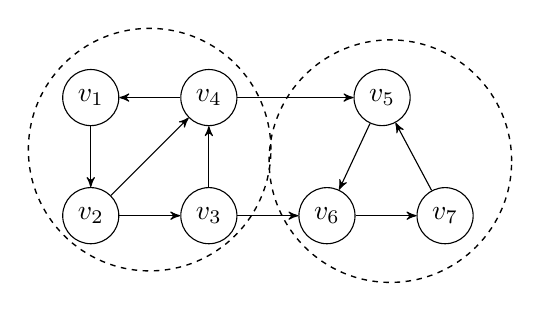
\begin{tikzpicture}[->, >=stealth', node distance=1.5cm, on grid, auto]
                                % Define the nodes
                                \node[circle,draw] (v1) {$v_1$};
                                \node[circle,draw] (v2) [circle, draw, below=of v1] {$v_2$};
                                \node[circle,draw] (v3) [circle, draw, right=of v2] {$v_3$};
                                \node[circle,draw] (v4) [circle, draw, right=of v1] {$v_4$};
                                \node[circle,draw] (v5) [circle, draw, right=2.2cm of v4] {$v_5$};
                                \node[circle,draw] (v6) [circle, draw, right=of v3] {$v_6$};
                                \node[circle,draw] (v7) [circle, draw, right=of v6] {$v_7$};

                                % Draw the edges
                                \draw[->] (v1) to (v2);
                                \draw[->] (v2) to (v4);
                                \draw[->] (v2) to (v3);
                                \draw[->] (v3) to (v4);
                                \draw[->] (v4) to (v1);
                                \draw[->] (v3) to (v6);
                                \draw[->] (v4) to (v5);
                                \draw[->] (v5) to (v6);
                                \draw[->] (v6) to (v7);
                                \draw[->] (v7) to (v5);

                                % Calculate the center point between v3, v4, and v6
                                \path (v2) -- (v3) node[midway] (center1) {};
                                \path (center1) -- (v4) node[midway] (final_center1) {};

                                \path (v6) -- (v7) node[midway] (center2) {};
                                \path (center2) -- (v5) node[midway] (final_center2) {};

                                % Offsets
                                \coordinate (adjusted_center1) at ($(final_center1)+(-0.2,0)$);
                                \coordinate (adjusted_center2) at ($(final_center2)+(0.2,0)$);

                                % Draw the dotted circles
                                \draw[dotted, line width=0.5pt, dash pattern=on 2pt off 2pt] (adjusted_center1) circle (1.54cm);
                                \draw[dotted, line width=0.5pt, dash pattern=on 2pt off 2pt] (adjusted_center2) circle (1.54cm);
                        \end{tikzpicture}\\ [3pt]
                \end{center}
                \textsc{ComponentiConnesse($G$)} $:\ O(|\textbf{V}|+|\textbf{E}|)$\\ [3pt]
                \verb| 1|\hspace*{0.5em} $\textbf{for each } v \in \textbf{V}$\\
                \verb| 2|\hspace*{1.5em} $v.etichetta \leftarrow -1$\\
                \verb| 3|\hspace*{0.5em} $eti \leftarrow 1$\\
                \verb| 4|\hspace*{0.5em} $\textbf{for each } v \in \textbf{V}$\\
                \verb| 5|\hspace*{1.5em} $\textbf{if } v.etichetta = -1$\\
                \verb| 6|\hspace*{2.5em} \textsc{VisitaEdEtichetta($G,v,eti$)}\\
                \verb| 7|\hspace*{2.5em} $eti \leftarrow eti + 1$\\ [5pt]
                \textsc{VisitaEdEtichetta} funziona come \textsc{VisitaAmpiezza} o \textsc{VisitaProfondità} ma imposta a $eti$ il campo $etichetta$ del nodo visitato. \\ [5pt]
                \textbf{Ordinamento topologico}\\ [3pt]
                L'\textit{ordinamento topologico} è una sequenza di nodi di un grafo \textit{orientato aciclico} tale per cui nessun nodo compare prima di un suo predecessore. \\ [3pt]
                \textbf{Esempio} \\ [3pt]
                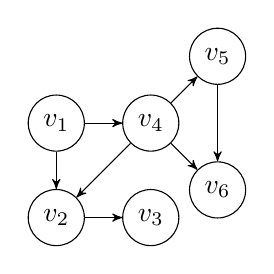
\begin{tikzpicture}[->, >=stealth', node distance=1.2cm, on grid, auto]

                        % Nodes for the graph on the left
                        \node (v1) [circle, draw] {$v_1$};
                        \node (v2) [circle, draw, below=of v1] {$v_2$};
                        \node (v4) [circle, draw, right=of v1] {$v_4$};
                        \node (v3) [circle, draw, below=of v4] {$v_3$};
                        \node (v5) [circle, draw, above right=of v4] {$v_5$};
                        \node (v6) [circle, draw, below right=of v4] {$v_6$};

                        % Edges for the graph on the left
                        \draw (v1) to (v4);
                        \draw (v1) to (v2);
                        \draw (v2) to (v3);
                        \draw (v4) to (v2);
                        \draw (v4) to (v5);
                        \draw (v4) to (v6);
                        \draw (v5) to (v6);

                \end{tikzpicture}\hfill
                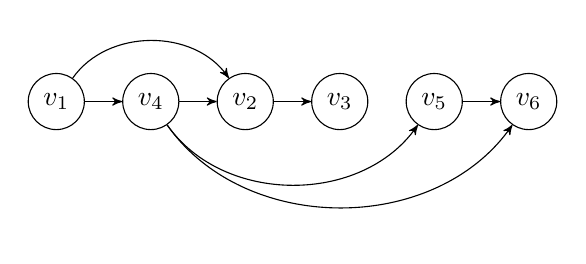
\begin{tikzpicture}[->, >=stealth', node distance=1.2cm, on grid, auto]

                        % Nodes for the sorted sequence on the right
                        \node (v1) [circle, draw] {$v_1$};
                        \node (v4) [circle, draw, right=of v1] {$v_4$};
                        \node (v2) [circle, draw, right=of v4] {$v_2$};
                        \node (v3) [circle, draw, right=of v2] {$v_3$};
                        \node (v5) [circle, draw, right=of v3] {$v_5$};
                        \node (v6) [circle, draw, right=of v5] {$v_6$};

                        % Edges for the sorted sequence on the right
                        \draw (v1) to [bend left=55] (v2);
                        \draw (v1) to (v4);
                        \draw (v4) to (v2);
                        \draw (v2) to (v3);
                        \draw (v4) to [bend right=55] (v5);
                        \draw (v4) to [bend right=55] (v6);
                        \draw (v5) to (v6);
                \end{tikzpicture}
                \begin{multicols}{2}
                        \textsc{OrdinamentoTopologico($G$)} \\ [3pt]
                        \verb| 1|\hspace*{0.5em} $\textbf{for each } v \in \textbf{V}$\\
                        \verb| 2|\hspace*{1.5em} $v.color \leftarrow white$\\
                        \verb| 3|\hspace*{0.5em} $\textbf{for each } v \in \textbf{V}$\\
                        \verb| 4|\hspace*{1.5em} $\textbf{if } v.color = white$\\
                        \verb| 5|\hspace*{2.5em} \textsc{VisitaProfOT($G,v,l$)}\\
                        \verb| 6|\hspace*{0.5em} \textbf{return $L$}\\
                        \columnbreak
                        \textsc{VisitaProfOT($G,s,L$)} \\ [3pt]
                        \verb| 1|\hspace*{0.5em} $s.color \leftarrow grey$\\
                        \verb| 2|\hspace*{0.5em} $\textbf{for each } v \in cur.adiacenti$\\
                        \verb| 3|\hspace*{1.5em} $\textbf{if } v.color = white$\\
                        \verb| 4|\hspace*{2.5em} $\textsc{VisitaProfOT($G,v,L$)}$\\
                        \verb| 5|\hspace*{0.5em} $s.color \leftarrow black$\\
                        \verb| 6|\hspace*{0.5em} $\textsc{PushFront($L,s$)}$\\
                \end{multicols}
                \textbf{Percorso più breve}\\ [3pt]
                Dato un grafo e un suo nodo $s$, individua i percorsi più brevi da $s$ a qualunque altro nodo. \\ [3pt]
                \textsc{DijkstraQueue($G,s$)} $: O((|\textbf{V}|+|\textbf{E}|)\log(|\textbf{V}|))$\\ [3pt]
                \verb| 1|\hspace*{0.5em} $Q \leftarrow \varnothing$\\
                \verb| 2|\hspace*{0.5em} $s.dist \leftarrow 0$\\
                \verb| 3|\hspace*{0.5em} $\textbf{for each } v \in |\textbf{V}|$\\
                \verb| 4|\hspace*{1.5em} $\textbf{if } v \ne s$\\
                \verb| 5|\hspace*{2.5em} $v.dist \leftarrow \infty$\\
                \verb| 6|\hspace*{2.5em} $v.pred \leftarrow NIL$\\
                \verb| 7|\hspace*{1.5em} $\textsc{AccodaPri($Q,v,v.dist$)}$\\
                \verb| 8|\hspace*{0.5em} $\textbf{while } Q \ne \varnothing$\\
                \verb| 9|\hspace*{1.5em} $u \leftarrow \textsc{CancellaMin($Q$)}$\\
                \verb|10|\hspace*{1.5em} $\textbf{for each } v \in u.succ$\\
                \verb|11|\hspace*{2.5em} $ndis \leftarrow u.dist + peso(u,v)$\\
                \verb|12|\hspace*{2.5em} $\textbf{if } v.dist > ndis$\\
                \verb|13|\hspace*{3.5em} $v.dist \leftarrow ndis$\\
                \verb|14|\hspace*{3.5em} $u.prev \leftarrow u$\\
                \verb|15|\hspace*{3.5em} \textsc{DecrementaPri($Q,v,ndis$)}\\ [5pt]
                \textbf{Rilevamento cicli (Floyd lepre e tartaruga)} \\ [5pt]
                Dato un grafo orientato, per cui ogni nodo ha un solo successore determina, dato un nodo di partenza $s$, se il cammino che parte da $s$ ha cicli. \\ [3pt]
                \textbf{Grafo di esempio} \\[3pt]
                \begin{center}
                        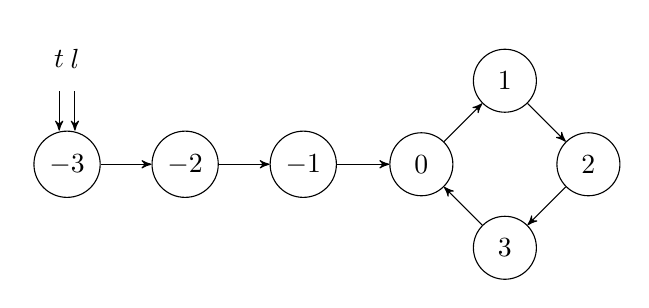
\begin{tikzpicture}[->, >=stealth', node distance=1.5cm, on grid, auto, every node/.style={minimum size=8mm} ]

                                \node (v1) [circle, draw] {$-3$};
                                \node (v2) [circle, draw, right=of v1] {$-2$};
                                \node (v3) [circle, draw, right=of v2] {$-1$};
                                \node (v4) [circle, draw, right=of v3] {$0$};
                                \node (v5) [circle, draw, above right=of v4] {$1$};
                                \node (v6) [circle, draw, below right=of v5] {$2$};
                                \node (v7) [circle, draw, below left=of v6] {$3$};

                                \draw (v1) to (v2);
                                \draw (v2) to (v3);
                                \draw (v3) to (v4);
                                \draw (v4) to (v5);
                                \draw (v5) to (v6);
                                \draw (v6) to (v7);
                                \draw (v7) to (v4);

                                \draw[->] ($(v1.north)+(-0.1,0.5)$) node [above] {$t$} to ($(v1.north)+(-0.1,0)$);
                                \draw[->] ($(v1.north)+(0.1,0.5)$) node [above] {$l$} to ($(v1.north)+(0.1,0)$);
                        \end{tikzpicture}
                \end{center}
                L'idea è quella di usare due riferimenti $t$ e $l$ che partono dal nodo iniziale $(-3 \text{ nell'esempio})$ che vengono spostati a ogni passo. Nello specifico, $t$ viene spostato dal nodo a cui punta al successore e $l$ viene spostato dal nodo a cui punta al successore del successore. È garantito che se c'è un ciclo, i due riferimenti si incontreranno. \\ [3pt]
                Sia $C$ la lunghezza del ciclo ($4$ nell'esempio) e $T$ la lunghezza della ``coda'' che lo precede (3 nell'esempio), allora l'algoritmo è il seguente: \\ [5pt]
                \textsc{FloydLT($G,x$)} $: \Theta(2(T+C)-r)$\\ [3pt]
                \verb| 1|\hspace*{0.5em} $t \leftarrow x.succ$\\
                \verb| 2|\hspace*{0.5em} $l \leftarrow x.succ.succ$\\
                \verb| 3|\hspace*{0.5em} \textbf{while} $l \ne t$\\
                \verb| 4|\hspace*{1.5em} $t \leftarrow t.succ$\\
                \verb| 5|\hspace*{1.5em} $l \leftarrow l.succ.succ$\\
                \verb| 6|\hspace*{0.5em} $T \leftarrow 0$\\
                \verb| 7|\hspace*{0.5em} $t \leftarrow x$\\
                \verb| 8|\hspace*{0.5em} \textbf{while} $l \ne t$\\
                \verb| 9|\hspace*{1.5em} $t \leftarrow t.succ$\\
                \verb|10|\hspace*{1.5em} $l \leftarrow l.succ$\\
                \verb|11|\hspace*{1.5em} $T \leftarrow T + 1$\\
                \verb|12|\hspace*{0.5em} $l \leftarrow t$\\
                \verb|13|\hspace*{0.5em} $C \leftarrow 0$\\
                \verb|14|\hspace*{0.5em} \textbf{while} $l \ne t$\\
                \verb|15|\hspace*{1.5em} $l \leftarrow l.succ$\\
                \verb|16|\hspace*{1.5em} $C \leftarrow C + 1$\\
                \verb|17|\hspace*{0.5em} \textbf{return} $T, C$\\ [5pt]
                \section{Algoritmi di ordinamento}
                \subsubsection{Bubble sort}
                Bubble Sort funziona passando ripetutamente attraverso l'array da ordinare, confrontando gli elementi adiacenti e scambiandoli se sono nell'ordine sbagliato. Prosegue attraverso l'array più volte fino a quando non sono più necessari scambi, indicando che l'array è ordinato. \\ [3pt]
                \textsc{BubbleSort($A$)} $: O(n^2)$\\ [3pt]
                \verb|1|\hspace*{0.5em} \textbf{for} $i \leftarrow 1$ \textbf{to} $A.length - 1$\\
                \verb|2|\hspace*{1.5em} \textbf{for} $j \leftarrow 1$ \textbf{to} $A.length - i$\\
                \verb|3|\hspace*{2.5em} \textbf{if} $A[j] > A[j + 1]$\\
                \verb|4|\hspace*{3.5em} \textsc{Swap}($A[j], A[j + 1]$)\\
                \subsubsection{Selection sort}
                Selection Sort seleziona ripetutamente l'elemento più piccolo dall'array non ordinato e lo scambia con l'elemento nella posizione corrente. Continua questo processo, aumentando progressivamente la porzione ordinata dell'array fino a quando l'intero array è ordinato. \\ [3pt]
                \textsc{SelectionSort($A$)} $: O(n^2)$\\ [3pt]
                \verb|1|\hspace*{0.5em} \textbf{for} $i \leftarrow 1$ \textbf{to} $A.length - 1$\\
                \verb|2|\hspace*{1.5em} $min\_index \leftarrow i$\\
                \verb|3|\hspace*{1.5em} \textbf{for} $j \leftarrow i + 1$ \textbf{to} $A.length$\\
                \verb|4|\hspace*{2.5em} \textbf{if} $A[j] < A[min\_index]$\\
                \verb|5|\hspace*{3.5em} $min\_index \leftarrow j$\\
                \verb|6|\hspace*{1.5em} \textsc{Swap}($A[i], A[min\_index]$)
                \subsubsection{Insertion sort}
                Insertion Sort costruisce l'array ordinato uno alla volta. Prende ciascun elemento dall'input e lo inserisce nella sua posizione corretta rispetto agli elementi già ordinati. Questo processo continua fino a quando l'intero array è ordinato. \\ [3pt]
                \textsc{InsertionSort($A$)} $: O(n^2)$\\ [3pt]
                \verb|1|\hspace*{0.5em} \textbf{for} $i \leftarrow 2$ \textbf{to} $A.length$\\
                \verb|2|\hspace*{1.5em} $tmp \leftarrow A[i]$\\
                \verb|3|\hspace*{1.5em} $j \leftarrow i - 1$\\
                \verb|4|\hspace*{1.5em} \textbf{while} $j \geq 1$ \textbf{and} $A[j] > tmp$\\
                \verb|5|\hspace*{2.5em} $A[j + 1] \leftarrow A[j]$\\
                \verb|6|\hspace*{2.5em} $j \leftarrow j - 1$\\
                \verb|7|\hspace*{1.5em} $A[j + 1] \leftarrow tmp$\\
                \subsubsection{Merge sort}
                Merge Sort è un algoritmo di divide et impera. Divide l'array di input in due metà, ordina ricorsivamente ciascuna metà e poi fonde le due metà ordinate in un singolo array ordinato. \\ [3pt]
                \begin{multicols}{2}
                        \textsc{MergeSort($A, p, r$)} $: \Theta(n\log n)$\\ [3pt]
                        \verb|1|\hspace*{0.5em} \textbf{if} $p < r - 1$\\
                        \verb|2|\hspace*{1.5em} $q \leftarrow \lfloor \frac{p + r}{2} \rfloor$\\
                        \verb|3|\hspace*{1.5em} \textsc{MergeSort}($A, p, q$)\\
                        \verb|4|\hspace*{1.5em} \textsc{MergeSort}($A, q + 1, r$)\\
                        \verb|5|\hspace*{1.5em} \textsc{Merge}($A, p, q, r$)\\
                        \verb|6|\hspace*{1.5em} \textbf{else if} $A[p] > A[r]$\\
                        \verb|7|\hspace*{2.5em} $tmp \leftarrow A[r]$\\
                        \verb|8|\hspace*{2.5em} $A[r] \leftarrow A[p]$\\
                        \verb|9|\hspace*{2.5em} $A[p] \leftarrow $ $tmp$\\
                        \columnbreak
                        \textsc{Merge($A, p, q, r$)} $: \Theta(n)$\\ [3pt]
                        \verb| 1|\hspace*{0.5em} $len_1 \leftarrow q - p + 1$\\
                        \verb| 2|\hspace*{0.5em} $len_2 \leftarrow r - q$\\
                        \verb| 3|\hspace*{0.5em} \textsc{Alloca}($L[1..len_1 + 1]$)\\
                        \verb| 4|\hspace*{0.5em} \textsc{Alloca}($R[1..len_2 + 1]$)\\
                        \verb| 5|\hspace*{0.5em} \textbf{for} $i \leftarrow 1$ \textbf{to} $len_1$\\
                        \verb| 6|\hspace*{1.5em} $L[i] \leftarrow A[p + i - 1]$\\
                        \verb| 7|\hspace*{0.5em} \textbf{for} $i \leftarrow 1$ \textbf{to} $len_2$\\
                        \verb| 8|\hspace*{1.5em} $R[i] \leftarrow A[q + i]$\\
                        \verb| 9|\hspace*{0.5em} $L[len_1 + 1] \leftarrow \infty$\\
                        \verb|10|\hspace*{0.5em} $R[len_2 + 1] \leftarrow \infty$\\
                        \verb|11|\hspace*{0.5em} $i \leftarrow 1$\\
                        \verb|12|\hspace*{0.5em} $j \leftarrow 1$\\
                        \verb|13|\hspace*{0.5em} \textbf{for} $k \leftarrow p$ \textbf{to} $r$\\
                        \verb|14|\hspace*{1.5em} \textbf{if} $L[i] \le R[j]$\\
                        \verb|15|\hspace*{2.5em} $A[k] \leftarrow L[i]$\\
                        \verb|16|\hspace*{2.5em} $i \leftarrow i + 1$\\
                        \verb|17|\hspace*{1.5em} \textbf{else}\\
                        \verb|18|\hspace*{2.5em} $A[k] \leftarrow R[j]$\\
                        \verb|19|\hspace*{2.5em} $j \leftarrow j + 1$\\
                \end{multicols}
                \subsubsection{Quick sort}
                Quick Sort è anch'esso un algoritmo di divide et impera. Sceglie un elemento pivot e suddivide l'array intorno a esso, in modo che gli elementi più piccoli del pivot siano a sinistra e quelli più grandi a destra. Ordina ricorsivamente le sotto-liste formate dalla partizione fino a quando l'intero array è ordinato. \\ [3pt]

                \myparagraph{Quick sort con schema di partizione di Lomuto}
                Lo schema di partizione di Lomuto seleziona l'ultimo elemento dell'array come pivot. Successivamente, scorre l'array e posiziona gli elementi più piccoli del pivot a sinistra e quelli più grandi a destra. Infine, sposta il pivot nella sua posizione corretta tra i due gruppi. \\

                \begin{multicols}{2}
                        \textsc{Quicksort($A, lo, hi$)}\\ [3pt]
                        \verb|1|\hspace*{0.5em} \textbf{se} $lo < hi$\\
                        \verb|2|\hspace*{1.5em} $p \leftarrow \textsc{PartLomuto}(A, lo, hi)$\\
                        \verb|3|\hspace*{1.5em} \textsc{Quicksort}($A, lo, p - 1$)\\
                        \verb|4|\hspace*{1.5em} \textsc{Quicksort}($A, p + 1, hi$)\\
                        \columnbreak
                        \textsc{PartLomuto($A, lo, hi$)}\\
                        \verb|1|\hspace*{0.5em} $pivot \leftarrow A[hi]$\\
                        \verb|2|\hspace*{0.5em} $i \leftarrow lo - 1$\\
                        \verb|3|\hspace*{0.5em} \textbf{for} $j \leftarrow lo$ \textbf{a} $hi - 1$\\
                        \verb|4|\hspace*{1.5em} \textbf{if} $A[j] \le pivot$\\
                        \verb|5|\hspace*{2.5em} $i \leftarrow i + 1$\\
                        \verb|6|\hspace*{2.5em} \textsc{Swap}($A[i], A[j]$)\\
                        \verb|7|\hspace*{0.5em} \textsc{Swap}($A[i + 1], A[hi]$)\\
                        \verb|8|\hspace*{0.5em} \textbf{return} $i + 1$\\
                \end{multicols}

                \myparagraph{Quick sort con schema di partizione di Hoare}
                Lo schema di partizione di Hoare seleziona il primo elemento dell'array come pivot. Utilizza due indici, uno che procede dall'inizio dell'array verso destra e uno che procede dalla fine dell'array verso sinistra, scambiando gli elementi fuori posizione fino a quando i due indici si incontrano. Alla fine, il pivot viene inserito tra i due gruppi e l'indice di partizione è determinato.
                \begin{multicols}{2}
                        \textsc{Quicksort($A, lo, hi$)}\\ [3pt]
                        \verb|1|\hspace*{0.5em} \textbf{se} $lo < hi$\\
                        \verb|2|\hspace*{1.5em} $p \leftarrow \textsc{PartHoare}(A, lo, hi)$\\
                        \verb|3|\hspace*{1.5em} \textsc{Quicksort}($A, lo, p$)\\
                        \verb|4|\hspace*{1.5em} \textsc{Quicksort}($A, p + 1, hi$)\\
                        \columnbreak
                        \textsc{PartHoare($A, lo, hi$)}\\ [3pt]
                        \verb| 1|\hspace*{0.5em} $pivot \leftarrow A[lo]$\\
                        \verb| 2|\hspace*{0.5em} $i \leftarrow lo - 1$\\
                        \verb| 3|\hspace*{0.5em} $j \leftarrow hi + 1$\\
                        \verb| 4|\hspace*{0.5em} \textbf{while true}\\
                        \verb| 5|\hspace*{1.5em} \textbf{repeat}\\
                        \verb| 6|\hspace*{2.5em} $j \leftarrow j - 1$\\
                        \verb| 7|\hspace*{2.5em} \textbf{until} $A[j] \le pivot$\\
                        \verb| 8|\hspace*{1.5em} \textbf{repeat}\\
                        \verb| 9|\hspace*{2.5em} $i \leftarrow i + 1$\\
                        \verb|10|\hspace*{2.5em} \textbf{until} $A[i] \ge pivot$\\
                        \verb|11|\hspace*{1.5em} \textbf{if} $i < j$\\
                        \verb|12|\hspace*{2.5em} \textsc{Swap}($A[i], A[j]$)\\
                        \verb|13|\hspace*{1.5em} \textbf{else return} $j$\\
                \end{multicols}
                Lo schema di partizione di Hoare effettua in media $\frac{1}{3}$ degli scambi effettuati dallo schema di partizione di Lomuto. (Entrambi hanno complessità $\Theta(n)$)
                \subsubsection{Heap sort}
                Heap Sort ordina l'array costruendo un max heap. Successivamente, estrae ripetutamente l'elemento massimo dall'heap e lo posiziona alla fine dell'array. Questo processo continua fino a quando l'intero array è ordinato. \\ [3pt]
                \textsc{HeapSort($A$)}: $\Theta(n \log n)$\\ [3pt]
                \verb|1|\hspace*{0.5em} \textsc{BuildMaxHeap}($A$)\\
                \verb|2|\hspace*{0.5em} \textbf{for} $i \leftarrow A.length$ \textbf{to} $2$\\
                \verb|3|\hspace*{1.5em} \textbf{swap} $(A[1],A[i])$\\
                \verb|4|\hspace*{1.5em} $A.heapsize \leftarrow A.heapsize - 1$\\
                \verb|5|\hspace*{1.5em} \textsc{MaxHeapify}($A, 1$)\\
                \subsubsection{Counting sort}
                Counting Sort è un algoritmo usato per ordinare un array di interi quando si conosce in anticipo il range dei valori possibili. Calcola un istogramma delle occorrenze di ciascun valore, quindi costruisce l'array ordinato posizionando ogni elemento nella sua posizione corretta basata sul conteggio accumulato degli elementi precedenti.
                \myparagraph{Non stabile}
                \textsc{CountingSort($A$)} $: O(n+k)$\\ [3pt]
                \verb|1|\hspace*{0.5em} $Ist[0..k] \leftarrow 0$\\
                \verb|2|\hspace*{0.5em} \textbf{for} $i \leftarrow 0$ \textbf{to} $A.length - 1$\\
                \verb|3|\hspace*{1.5em} $Ist[A[i]] \leftarrow Ist[A[i]] + 1$\\
                \verb|4|\hspace*{0.5em} $idxA \leftarrow 0$\\
                \verb|5|\hspace*{0.5em} \textbf{for} $i \leftarrow 0$ \textbf{to} $k$\\
                \verb|6|\hspace*{1.5em} \textbf{while} $Ist[i] > 0$\\
                \verb|7|\hspace*{2.5em} $A[idxA] \leftarrow i$\\
                \verb|8|\hspace*{2.5em} $idxA \leftarrow idxA + 1$\\
                \verb|9|\hspace*{2.5em} $Ist[i] \leftarrow Ist[i] - 1$
                \myparagraph{Stabile}
                \textsc{CountingSort($A$)} $: O(n+k)$\\ [3pt]
                \verb| 1|\hspace*{0.5em} $B[0..A.length - 1] \leftarrow 0$\\
                \verb| 2|\hspace*{0.5em} $Ist[0..k] \leftarrow 0$\\
                \verb| 3|\hspace*{0.5em} \textbf{for} $i \leftarrow 0$ \textbf{to} $A.length - 1$\\
                \verb| 4|\hspace*{1.5em} $Ist[A[i]] \leftarrow Ist[A[i]] + 1$\\
                \verb| 5|\hspace*{0.5em} $sum \leftarrow 0$\\
                \verb| 6|\hspace*{0.5em} \textbf{for} $i \leftarrow 0$ \textbf{to} $k$\\
                \verb| 7|\hspace*{1.5em} $sum \leftarrow sum + Ist[i]$\\
                \verb| 8|\hspace*{1.5em} $Ist[i] \leftarrow sum$\\
                \verb| 9|\hspace*{0.5em} \textbf{for} $i \leftarrow A.length - 1$ \textbf{to} $0$\\
                \verb|10|\hspace*{1.5em} $idx \leftarrow Ist[A[i]]$\\
                \verb|11|\hspace*{1.5em} $B[idx - 1] \leftarrow A[i]$\\
                \verb|12|\hspace*{1.5em} $Ist[A[i]] \leftarrow Ist[A[i]] - 1$\\
                \verb|13|\hspace*{0.5em} \textbf{return} $B$
                \subsection{Confronto}
                Confronto delle complessità temporali e spaziali degli algoritmi di ordinamento: \\ [5pt]
                \renewcommand{\arraystretch}{1.5}%
                \begin{tabular}{l|>{\centering\arraybackslash}m{1cm}|m{2.2cm}|m{2.3cm}|>{\centering\arraybackslash}m{1.1cm}}
                        Algoritmo & Stabile?     & $T(n)$ (pessimo)                             & $T(n)$ (ottimo)                             & $S(n)$      \\
                        \hline
                        Bubble    & $\checkmark$ & $\Theta(n^2)$\hfill (\textbf{\textit{inv.}}) & $\Theta(n)$\hfill  (\textbf{\textit{ord.}}) & $O(1)$      \\
                        \hline
                        Selection & $\times$     & $\Theta(n^2)$                                & $\Theta(n^2)$                               & $O(1)$      \\
                        \hline
                        Insertion & $\checkmark$ & $\Theta(n^2)$ \hfill(\textbf{\textit{inv.}}) & $\Theta(n)$ \hfill (\textbf{\textit{ord.}}) & $O(1)$      \\
                        \hline
                        Merge     & $\checkmark$ & $\Theta(n \log n)$                           & $\Theta(n \log n)$                          & $\Theta(n)$ \\
                        \hline
                        Quick     & $\times$     & $\Theta(n^2)$ \hfill(\textbf{\textit{ord.}}) & $\Omega(n \log n)$                          & $O(1)$      \\
                        \hline
                        Heap      & $\times$     & $\Theta(n \log n)$                           & $\Theta(n\log n)$                           & $O(1)$      \\
                        \hline
                        Counting  & $\checkmark$ & $O(n + k)$                                   & $O(n + k)$                                  & $O(n + k)$  \\
                \end{tabular}\\ [5pt]
                \textbf{N.B.} Il quick sort nel caso medio ha complessità $\Theta(n\log n)$
        \vfill
\end{multicols*}
\end{document}
